\chapter{Partitives and part-whole structures}\label{ch:partitives-and-part-whole-structures}

In this chapter, I will examine cross-linguistic evidence for the relevance of subatomic quantification in natural language. In particular, I will focus on the distribution and semantic properties of distinct types of partitives some of which have not received much attention in the linguistic literature oriented towards the study of meaning. Specifically, I will investigate constructions involving proportional expressions such as \textit{part} and \textit{half} in order to reveal some non-trivial facts about partitivity. I will provide novel data indicating that singulars and plurals share one unified parthood relation. Furthermore, I will show that distinct part-whole structures result from the fact that certain entities are conceptualized as cohesive individuals whereas others are not. Crucially, the distinction turns out to be relevant from the perspective of countability. In particular, partitive constructions indicate that cardinal numerals select only for predicates denoting entities conceptualized as integrated wholes.\footnote{I would like to sincerely thank my informants with whom I have consulted the structures and meanings of particular constructions. Specifically, many thanks to Muriel Assmann, Katie Fraser, Berit Gehrke, Nina Haslinger, Aitor Lizardi Ituarte, Tetiana Kamyshanova, Radvan Markus, Erlinde Meertens, Lilla Pintér, Martin Prinzhorn, Adam Przepiórkowski, Viola Schmitt, Hana Strachoňová, Yasutada Sudo, Balázs Surányi, Peter Sutton, and Guy Tabachnick. Finally, I am deeply grateful to Enrico Flor and Chiara Masnovo for their judgments and the discussion of the Italian data. Their introspective reports and insightful comments were of invaluable help for the relevant parts of this chapter.}

\section{Partitives}\label{sec:partitives}

As already mentioned in the introduction, the part-whole relation is an important notion in human cognition and natural language. For instance, large parts of the lexicon are structured by means of meronymy, i.e., the relation that holds between expressions denoting entities conceptualized as whole objects (holonyms) and expressions denoting parts of such wholes (meronyms), e.g., the relationship between \textit{cat} and \textit{tail}. However, the relevance of partitivity in natural language is not restricted to lexical associations but it is also reflected in grammar. As noticed by \citet{hoeksema1996introduction}, its importance for the syntax-semantics interface is corroborated by the fact that the link between a whole and its parts can support definite descriptions, as witnessed in \ref{ex:partitivity-definites}.

\ex. English \citep[p. 1]{hoeksema1996introduction}
\b.[] I still have a jar of gooseberry jam, but I cannot get the lid off.\label{ex:partitivity-definites}

There are many ways in which the part-whole relation can be expressed syntactically and languages differ in what means they employ in order to indicate it. Sometimes even though a particular construction lacks a formal exponent expressing partitivity, the relation between the elements is well understood. For example, English compounds lack morphological means to express partitivity, but often the part-whole relation between the referents of the first stem and the referents of the second stem is semantically transparent and can be readily retrieved, as in \ref{ex:english-compounds} \citep{hoeksema1996introduction}.

\ex. English \citep[p. 1]{hoeksema1996introduction}\label{ex:english-compounds}
\a. chicken-feet
\b. church-door
\b. mountain-top

In this book, however, I will restrict my focus to the structure that expresses the part-whole relation formally, i.e. the so-called partitive construction. The partitive is an expression of natural language that indicates partialness. In English, nominal partitives commonly take the form as in \ref{ex:paritive-form}.\footnote{The structure in \ref{ex:paritive-form} is just one possible analysis. In fact, there are several different proposals concerning the syntax of partitives. For instance \citet{ionin_matushansky_ruys2006parts} argue for different structures for distinct types of partitives, see \ref{ex:different-partitives-ionin-et-al}. However, for the most part I will ignore all the syntactic intricacies here.

\ex. English \citep{ionin_matushansky_ruys2006parts}\label{ex:different-partitives-ionin-et-al}
\a. [$_{\text{NP}}$ half [$_{\text{PP}}$ of [$_{\text{DP}}$ these [$_{\text{NP}}$ eight apples]]]]\label{ex:proportional-partitives-ionin-et-al}
\b. [$_{\text{NP}}$ two [$_{\text{NP}}$ $\varnothing$/\sout{apple} [$_{\text{PP}}$ of [$_{\text{DP}}$ these [$_{\text{NP}}$ eight apples]]]]]\label{ex:count-partitives-ionin-et-al}

}

\ex. Partitive structure \citep{marti_i_girbau2010syntax}\label{ex:paritive-form}
\a. [$_{\text{DP}}$ Det [$_{\text{PP}}$ of [$_{\text{DP}}$ Det NP]]]
\b. [three [of [my friends]]] 

The upstairs determiner is a quantifier, whereas the preposition \textit{of} links it with the larger whole denoted by its complement, i.e., the embedded definite or specific DP, from which it is partitioned. A similar frame is found in many other Germanic languages as well as in Romance, as demonstrated in \ref{ex:partitives-germanic} and \ref{ex:partitives-romance}.

\ex. Dutch
\bg.[] drie van mijn vrienden\label{ex:partitives-germanic}\\
three of my friends\\

\ex.French
\bg.[] trois de mes amis\label{ex:partitives-romance}\\
three of my friends\\

On the other hand, in languages such as Estonian and Finnish, a special partitive case can be used instead of the prepositional element, see \ref{ex:partitives-paritive-case} \citep{de_hoop2003partitivity}, whereas, e.g., German and many Slavic languages can express the partitive with the genitive (the so-called partitive genitive), see \ref{ex:partitives-genitive-case} (see, e.g., \citealt{hoeing1997phrase} for German and \citealt{valkova1999semantics,rutkowski2007syntactic} for Slavic).\footnote{Notice, however, that Finnish also has another construction in which the embedded noun appears in the elative case, as in \ref{ex:partitives-elative}. For more examples and discussion, see \citet{anttila_fong2000partitive}.

\ex. Finnish \citep[p. 111]{karlsson1999finnish}
\bg.[] viisi nais-i-sta\\
five woman-\textsc{pl}-\textsc{ela}\\
`five of the women'\label{ex:partitives-elative}

}

\ex. Finnish \citep{de_hoop2003partitivity}
\bg.[] Anne joi maitoa.\label{ex:partitives-paritive-case}\\
Anne drank milk\textsc{.part}\\
`Anne drank (some) milk.'

\ex. Russian
\bg.[] Oleg vypil polovinu moloka.\label{ex:partitives-genitive-case}\\
Oleg drank half milk\textsc{.gen}\\
`Oleg drank half the milk.'

In terms of meaning, the partitive picks out a part from a whole. The part is associated with the upstairs quantifier, whereas the whole is denoted by the embedded DP and can be either a singular entity or a plurality \citep[e.g.,][]{jackendoff1977x-bar,selkirk1977some,ladusaw1982semantic}. Thus, partitives can denote parts of individuals, see \ref{ex:entity-partitive}, as well as subsets of larger sets of individuals, see \ref{ex:set-partitive}, and portions of substances, see \ref{ex:mass-partitive}.\largerpage

\ex. English
\a. most of the apple\label{ex:entity-partitive}
\b. most of the apples\label{ex:set-partitive}
\b. most of the juice\label{ex:mass-partitive}

	An important observation concerning partitive constructions is that not every kind of DP can be embedded within the structure. A restriction called the Partitive Constraint excludes certain expressions from this position \citep[e.g.,][]{jackendoff1977x-bar,selkirk1977some,barwise_cooper1981generalized,ladusaw1982semantic}. In particular, its early formulations posited that only definites can appear in the downstairs DP.\footnote{See \citet{abbott1996doing} for a discussion and a proposal of an analysis not involving the Partitive Constraint.} Later approaches redefined the restriction in semantic terms postulating that the embedded DP needs to denote an entity, i.e., it needs to be either definite or specific \citep{de_hoop1997semantic}.

Before I begin a detailed discussion of the relationship between partitivity and countability it will be useful to make several terminological remarks. First, I will use the terms \textsc{part-words} and \textsc{half-words} to refer to expressions such as English \textit{part} and \textit{half}, respectively. Despite significant syntactic differences between those lexical items suggesting more fine-grained categorial distinctions, they both can appear in the upstairs Det position in partitives like \ref{ex:entity-partitive}, on a par with quantifiers such as \textit{most} and \textit{all}. From a cross-linguistic perspective different types of half-words often fall into different syntactic categories. For instance, German \textit{Hälfte} `half$_1$' appears to have nominal properties, whereas \textit{halb} `half$_2$' is a standard adjective. As demonstrated in \ref{ex:german-halfte}--\ref{ex:german-halb}, while \textit{Hälfte} has a gender value and either assigns the genitive case or combines with the prepositional \textit{von}-phrase assigning the dative (\citealt{durrell1996hammers}; see also \citealt{hoeing1997phrase,asbury2007towards} for the discussion of the structures), \textit{halb} agrees with the modified nouns. 

\ex.\label{ex:german-halfte-halb} German
\ag. eine Hälfte des Apfels\label{ex:german-halfte}\\
a\textsc{.nom.sg.f} half$_{1}$\textsc{.nom.f} the\textsc{.gen.sg.m} apple\textsc{.gen.m}\\
`a half of the apple'
\bg. eine Hälfte vom Apfel\label{ex:german-halfte-von}\\
a\textsc{.nom.sg.f} half$_{1}$\textsc{.nom.f} of.the\textsc{.dat.sg.m} apple\textsc{.dat.m}\\
`a half of the apple'
\bg. ein halber Apfel\label{ex:german-halb}\\
a\textsc{.nom.sg.m} half$_{2}$\textsc{.nom.m} apple\textsc{.nom.m}\\
`half an apple'

Since this book is primarily concerned with semantic aspects of partitivity, I take the terms part-word and half-word introduced above to refer to expressions explicitly designating a part of a whole. Therefore, despite the different syntactic structures expressions such as \textit{Hälfte} and \textit{halb} occur in, I will treat them as semantically related linguistic objects. The general term \textsc{partitive words} will be used to cover part-words and half-words as well as different types of proportional quantifiers that can be found in partitives.\footnote{The term more or less corresponds to what \citeauthor{quirk_greenbaum_leech_svartvik1985comprehensive} (\citeyear[p. 249]{quirk_greenbaum_leech_svartvik1985comprehensive}) call general partitive nouns excluding measure terms.}

Another issue concerns the grammatical number of the downstairs DP in the partitive construction. There is a tradition in the literature on partitivity to distinguish between partitive expressions referring to a portion of a singular entity and those referring to a subset of a set of individuals. The former are often called mass partitives and the latter group partitives \citep[e.g.,][]{hoeksema1996introduction,abbott1996doing}. However, despite this tradition I will follow \citet{de_hoop1997semantic,de_hoop2003partitivity} and refer to phrases such as \ref{ex:entity-partitive} as \textsc{entity partitives} and to phrases such as \ref{ex:set-partitive} as \textsc{set partitives}.\footnote{Yet another term is used by \citet{korat2016singular} to refer to partitives involving regular count singular nouns as well as collective nouns, namely singular quantified terms. However, since I do not focus on group nouns in this book, I will ignore the potential distinction.} Typically, entity partitives involve a singular term in the embedded DP, whereas set partitives comprise a quantifier combining with a plural DP. I will restrict the use of the term \textsc{mass partitives} to constructions such as \ref{ex:mass-partitive} where the upstairs determiner combines with the \textit{of}-phrase taking a mass term as its complement. The main reason is that I found the terms mass and group partitives confusing in that they suggest a correspondence with the mass/count distinction, contrary to fact \citep[see also][]{marti_i_girbau2010syntax}.

Furthermore, I will refer to constructions involving an overt part-word such as those in \ref{ex:explicit-partitive} as \textsc{explicit partitives}. On the other hand, I will call phrases containing proportional quantifiers such as \textit{most} or \textit{half}, see \ref{ex:proportional-partitive}, \textsc{proportional partitives}, whereas those involving fractions, see \ref{ex:fraction-partitive}, will be referred to as \textsc{fraction partitives}.

\ex. English
\a. part of the apple\label{ex:explicit-partitive}
\b. half of the apple\label{ex:proportional-partitive}
\b. two thirds of the apple\label{ex:fraction-partitive}

Finally, I will use the terms \textsc{count explicit partitives} and \textsc{count proportional partitives} to refer to phrases such as \ref{ex:count-explicit-partitive} and \ref{ex:count-proportional-partitive}, respectively, where the partitive word is modified by the cardinal numeral. These should not be confused with \textsc{count partitives}, the term sometimes used for phrases such as \ref{ex:count-partitives} \citep[e.g.,][]{ionin_matushansky_ruys2006parts}.\footnote{\citeauthor{quirk_greenbaum_leech_svartvik1985comprehensive} (\citeyear[p. 249]{quirk_greenbaum_leech_svartvik1985comprehensive}) call them plural partitives.}

\ex. English
\a. two parts of the apple\label{ex:count-explicit-partitive}
\b. two halves of the apple\label{ex:count-proportional-partitive}
\b. two of the apples\label{ex:count-partitives}

The next sections of this chapter will be dedicated to the interaction between cardinal numerals and partitives involving different types of expressions both in the upstairs DP head as well as in the embedded DP.

\section{The analogy}\label{sec:the-analogy}

At least since \citet{link1983logical} it is often assumed that it is necessary to distinguish between two distinct yet corresponding part-whole structures employed in natural language, namely one corresponding to the material constitution of objects and one capturing collections of distinct objects. Hence, the material part relation provides ordering for structures representing the relationship between portions of matter and individuals made out of that matter, whereas the individual part relation concerns particular objects and sums thereof. The distinction is motivated by the fact that things and stuff they consist of are apparently differentiated in natural language. The famous example concerns two golden rings. If they were forged recently out of some old Egyptian gold, then it is definitely true to state that the rings are new although the gold is old. 

However, there are some data that might be interpreted as suggesting that at least in some expressions natural language semantics does not distinguish between the two distinct part relations postulated by \citet{link1983logical} and instead employs a unified part-whole structure for different types of nominal expressions. \citet{moltmann1997parts,moltmann1998part} observes an analogy between partitives involving singular and plural terms. For instance, in German the same expression \textit{Teil} `part' can be used both in entity and set partitive constructions in order to quantify over parts of singular individuals and subsets of groups of individuals, see \ref{ex:analogy-entity-set-german}--\ref{ex:analogy-entity-set-german-von}.\footnote{In fact, \citet{moltmann1997parts,moltmann1998part} provides English examples to argue for her point, see \ref{ex:moltmann-unreliable}. However, since the reported felicity judgments for English contrast with Moltmann's claim \citep[see][]{schwarzschild1996pluralities}, I use the uncontroversial German examples in \ref{ex:analogy-entity-set-german}--\ref{ex:analogy-entity-set-german-von} instead.

\ex.\label{ex:moltmann-unreliable} English \citep[p. 11]{moltmann1997parts}
\a. \{all of / some of / part of\} the book
\b. \{all of / some of / part of\} the wine
\b. \{all of / some of / part of\} the books

} 

			\ex.\label{ex:analogy-entity-set-german} German (Nina Haslinger, p.c.)
            \ag. ein Teil des Apfels\label{ex:analogy-entity-german}\\
			a part the\textsc{.gen} apple\textsc{.gen}\\
			`(a) part of the apple'
			\bg. ein Teil der Äpfel\label{ex:analogy-set-german}\\
			a part the\textsc{.gen} apples\textsc{.gen}\\
			`some of the apples'
			
			\ex.\label{ex:analogy-entity-set-german-von} German (Nina Haslinger, p.c.)
            \ag. ein Teil vom Apfel\label{ex:analogy-entity-german-von}\\
			a part of.the\textsc{.dat} apple\textsc{.dat}\\
			`(a) part of the apple'
			\bg. ein Teil von den Äpfeln\label{ex:analogy-set-german-von}\\
			a part of the\textsc{.dat} apples\textsc{.dat}\\
			`some of the apples'

In particular, when used in the entity partitive, \textit{Teil} quantifies over material parts of singular objects, i.e., functional parts or portions of a substance making up the whole individual. For instance, \ref{ex:analogy-entity-german} and \ref{ex:analogy-entity-german-von} denote a set of parts of the relevant apple. It could be used to refer, e.g., to the stem end of the apple in question or its blossom end as well as its pulp or pips. On the other hand, when \textit{Teil} takes the plural DP as its complement, it quantifies over whole individuals, e.g., \ref{ex:analogy-set-german} and \ref{ex:analogy-set-german-von} make reference to a part of a particular collection, i.e., a subset of the apples rather than to a set of arbitrary parts of singular apples. For instance, given a situation in which there are three relevant apples $a_1$, $a_2$, and $a_3$, \ref{ex:analogy-set-german} and \ref{ex:analogy-set-german-von} could not be used to refer to a set involving the stem end of $a_1$ and a pip of $a_2$. Instead, it would be true of a set of some of the apples in question, e.g., a set comprising $a_1$ and $a_2$.

Notice that in German there is yet another interpretation an expression such as \ref{ex:analogy-set-german} and \ref{ex:analogy-set-german-von} can get. For instance, consider the two possible readings of \ref{ex:analogy-inverse-linking-german}. 

\ex. German (Nina Haslinger, p.c.)\label{ex:analogy-inverse-linking-german}
\bg.[] Ein kleiner Teil von den zehn Äpfeln ist schimmlig.\\
 a small part of the\textsc{.dat} ten apples\textsc{.dat} is moldy\\
 `A minority of the ten apples are moldy.' or\\
 `A small part of each of the ten apples is moldy.'

The sentence in \ref{ex:analogy-inverse-linking-german} would definitely be true in a situation where there are ten apples and two of them are completely moldy. Yet, there is also a different scenario where uttering \ref{ex:analogy-inverse-linking-german} would be truthful, namely if there were ten apples and each apple had a small patch of mold. At first blush, this behavior might appear to contradict what I claimed in the previous paragraph. However, there are good reasons to assume that this reading is independent from the two discussed above and results from a silent distributivity operator. Notice that the sentence would be judged false in a scenario where there were ten apples seven of which had a small patch of mold, whereas the others were not moldy. This shows that German explicit set partitives such as \ref{ex:analogy-set-german-von} have another interpretation in addition to the subset reading discussed above. Crucially, this interpretation does not involve quantification over arbitrary material parts. Rather, the definite seems to have a distributive interpretation with wide scope over the indefinite. Though it was important to draw the distinction between the two possible interpretations, I will ignore this additional distributive reading in the remaining part of this chapter.\footnote{In fact, this interpretation might turn out to be a German idiosyncrasy since it seems to be unavailable in some other languages, e.g., in Polish. Though it is an interesting issue on its own, which would require a systematic cross-linguistic survey, this book is about something different.}

Thus, it appears that the same expression can form either an entity partitive or a set partitive depending on the number value on its complement. This phenomenon seems intriguing and might imply a puzzle with respect to a proper treatment of German explicit partitives. But is it just a German idiosyncrasy? Or does the data in \ref{ex:analogy-entity-set-german}--\ref{ex:analogy-entity-set-german-von} actually reveal something deep about the way the human mind conceptualizes the difference between objects and collections of objects? And if so, to what extent is such a difference relevant for the semantic distinction between singularities and pluralities outside the domain of partitivity? I believe that, if approached in a systematic manner, an attempt to provide answers to these questions can shed new light on what it means to be an individuated entity and, as we will see, what it means to be countable.

Prima facie, it seems that there are two ways in which one could account for the phenomenon in question. A radical solution is to conclude that the data in \ref{ex:analogy-entity-set-german}--\ref{ex:analogy-entity-set-german-von} suggest a unified parthood structure for both singular and plural individuals across the board \citep{moltmann1997parts,moltmann1998part}. In other words, it is to posit that singularities and pluralities are in fact much less distinct than standardly assumed. On such an approach, the relationship between an object and its parts would be the same relationship as the one holding between a collection of objects and objects being part of that collection. Another way to explain the analogy would be to assume that partitive expressions such as \textit{Teil} employ a derived notion of parthood which generalizes over two distinct yet corresponding part-structures \citep{barker1998partitives,ionin_matushansky_ruys2006parts}. 

In the next section, I will present novel evidence indicating the source of the analogy in question. I will argue that the data to be examined suggests non-trivial implications for the part-whole structures that singular and plural expressions employ.

\subsection{Ambiguity or indeterminacy}\label{sec:ambiguity-or-indeterminacy}

The data we began with in \ref{ex:analogy-entity-set-german}--\ref{ex:analogy-entity-set-german-von} might be interpreted as suggesting that both singulars and plurals employ a unified part-whole structure. Another way of looking at the evidence involves preserving distinct mereologies and at the same time postulating that partitive words are either ambiguous between two different meanings or that they encode a generalized parthood relation which enables them to operate on both part-whole structures. A question I will attempt to tackle in this section concerns the one as to what extent there is an empirical basis broad enough to provide a solid argument in favor of one of the approaches. In particular, I will propose an independent test whose results provide evidence against the ambiguity account.

A standard diagnostic to detect ambiguity is the so-called zeugma test (\citealt{lasersohn1995plurality}; see also \citealt{zwicky_sadock1975ambiguity}). The test works as follows. The examined lexical item is put in a syntactic configuration with a coordination structure. If the expression in question is in fact ambiguous, then it must take the same interpretation with respect to both conjuncts. Otherwise the zeugma effect arises, i.e., the sentence takes on the flavor of a joke. On the other hand, if the tested item is unspecific or indeterminate, it can take different interpretations with respect to different conjuncts without any hilarious effect.

To illustrate this, let us consider the two examples in \ref{ex:zeugma-test}. 

\ex.\label{ex:zeugma-test} English \citep[p. 94; adapted]{lasersohn1995plurality} 
\a. John rented a car and a house.\label{ex:zeugma-test-ambiguous}
\b. John described a car and a house.\label{ex:zeugma-test-unambiguous}

The verb \textit{rent} must have the same interpretation with respect to both DPs, \textit{a car} and \textit{a house}, i.e., it is either the case that John owned a car and a house and he rented them out to someone, or it is the case that John rented a car and a house from someone. But crucially it cannot be the case that John rented out a car and rented a house as a tenant or vice versa. Therefore, since \textit{rent} must have the same interpretation with respect to the DPs \textit{a car} and \textit{a house}, it is ambiguous between the two described readings. On the other hand, the verb \textit{describe} in \ref{ex:zeugma-test-unambiguous} is indeterminate with respect to whether describing is done in speech or in writing. Since it is perfectly natural to understand the sentence in a way implying that John described a car in speech, whereas he described a house in writing, \textit{describe} is not ambiguous but rather merely unspecific.

The zeugma test has been used commonly in the study of natural language semantics including the research on pluralities \citep[see, e.g.,][]{dowty1987collective,lasersohn1995plurality,nouwen2016plurality}.\footnote{However, \citet[p. 95]{lasersohn1995plurality} points out that in fact the zeugma test does not detect ambiguity, but rather it reveals whether a particular item always makes the same contribution to the proposition. I will leave the issue as to whether \citeauthor{lasersohn1995plurality}'s objection stands open though.} Let us then examine whether part-words are ambiguous between two different readings giving rise to a part-of-a-singularity reading in entity partitives, on the one hand, and to a part-of-a-singularity reading in set partitives, on the other, or, alternatively, they are merely indeterminate in this respect. To this end, let us first consider the well-formed and felicitous German sentences in \ref{ex:zeugma-test-part-german-setup}. 

\ex.\label{ex:zeugma-test-part-german-setup} German (Viola Schmitt, Martin Prinzhorn, p.c.)
\ag. Ein Teil des Apfels und der Birne sind verfault.\label{ex:zeugma-test-part-sg-german-setup}\\
a part the\textsc{.gen} apple\textsc{.gen} and the\textsc{.gen} pear\textsc{.gen} are rotten\\
`Part of the apple and the pear got spoiled.'
\bg. Ein Teil der Birnen und der Äpfel sind verfault.\label{ex:zeugma-test-part-pl-german-setup}\\
a part the\textsc{.gen} pears\textsc{.gen} and the\textsc{.gen} apples\textsc{.gen} are rotten\\
`Some of the pears and the apples got spoiled.'

In the explicit entity partitive in \ref{ex:zeugma-test-part-sg-german-setup} the partitive word \textit{Teil} `part' takes a structure involving coordination of two singular DPs as a complement. As witnessed by the translation, the meaning of the sentence involves material partitivity, i.e., quantification over parts of the relevant singular objects, namely the apple and the pear. In other words, \ref{ex:zeugma-test-part-sg-german-setup} would be true if part of the apple and part of the pear got spoiled. On the other hand, \textit{Teil} in \ref{ex:zeugma-test-part-pl-german-setup} combines with a conjoined phrase involving two plural conjuncts. In this case, \textit{Teil} quantifies over parts of pluralities, i.e., the whole sentence designates that a subset of the apples and a subset of the pears got spoiled.

Now let us consider the interaction between \textit{Teil} and a coordinate structure conjoining a singular and a plural DP, as in \ref{ex:zeugma-test-part-german}. 

\ex.\label{ex:zeugma-test-part-german} German (Viola Schmitt, Martin Prinzhorn, p.c.)
\ag. Ein Teil des Apfels und der Birnen sind verfault.\label{ex:zeugma-test-part-sg-pl-german}\\
a part the\textsc{.gen} apple\textsc{.gen} and the\textsc{.gen} pears\textsc{.gen} are rotten\\
`Part of the apple and some of the pears got spoiled.'
\bg. Ein Teil der Birnen und des Apfels sind verfault.\label{ex:zeugma-test-part-pl-sg-german}\\
a part the\textsc{.gen} pears\textsc{.gen} and the\textsc{.gen} apple\textsc{.gen} are rotten\\
`Some of the pears and part of the apple got spoiled.'

The assumption behind \ref{ex:zeugma-test-part-german} is that if \textit{Teil} were merely indeterminate with respect to a part-of-a-singularity and part-of-a-plurality reading, it should be able to take the former interpretation with respect to the first conjunct and the latter interpretation with respect to the second conjunct in \ref{ex:zeugma-test-part-sg-pl-german} and vice versa in \ref{ex:zeugma-test-part-pl-sg-german}. On the other hand, if it were ambiguous between two different meanings such behavior should not be possible. Interestingly, \textit{Teil} not only can combine felicitously with a construction involving coordination of a singular and plural DP, but also irrespective of the linear order of the conjuncts, see \ref{ex:zeugma-test-part-sg-pl-german} and \ref{ex:zeugma-test-part-pl-sg-german}, it can take simultaneously two different readings.

The very same effect arises in \ref{ex:zeugma-test-part-german-sg.tant}, where one of the conjuncts is a singulare tantum noun, specifically the object mass noun \textit{Geschirr} `tableware' can refer either to one piece of tableware or to a collection thereof. 

\ex.\label{ex:zeugma-test-part-german-sg.tant} German (Viola Schmitt, Martin Prinzhorn, p.c.)
\ag. Ein Teil des Geschirrs und des Spülbeckens sind verrostet.\label{ex:zeugma-test-part-sg-sg.tant-german-sg.tant}\\
a part the\textsc{.gen} tableware\textsc{.gen} and the\textsc{.gen} sink\textsc{.gen} are rusted\\
`Some of the tableware and part of the kitchen sink got rusted.'
\bg. Ein Teil des Spülbeckens und des Geschirrs sind verrostet.\label{ex:zeugma-test-part-sg.tant-sg-german-sg.tant}\\
a part the\textsc{.gen} sink\textsc{.gen} and the\textsc{.gen} tableware\textsc{.gen} are rusted\\
`Part of the kitchen sink and some of the tableware got rusted.'

Both \ref{ex:zeugma-test-part-sg-sg.tant-german-sg.tant} and \ref{ex:zeugma-test-part-sg.tant-sg-german-sg.tant} are felicitous and they both can get the intended meaning, i.e., \textit{Teil} can simultaneously quantify over material parts of the kitchen sink and over individual items making up the tableware. Hence, the mismatch between the values of grammatical number on conjunct nominals in \ref{ex:zeugma-test-part-german} definitely does not play a role here and the effect seems to be purely semantic.\largerpage

At this point, a conclusion can be drawn. Given the results of the zeugma test, I deduce that part-words in German are not ambiguous between two different interpretations. Rather, they are semantically underspecified in the sense that their meaning is general enough to cover configurations involving both material and individual parthood. As a result a part-of-a-singularity understanding is derived in entity partitives whereas a part-of-a-plurality understanding arises in set partitives.

Having identified the source of the analogy between entity and set partitives, let us now examine to what extent it is valid from a wider cross-linguistic perspective.

\subsection{Entity and set partitives across languages}\label{sec:entity-and-set-partitives-across-languages}

For some reason, the analogy between explicit entity and set partitives does not hold in English. As observed by \citet[pp. 165--166]{schwarzschild1996pluralities}, there is a contrast between \ref{ex:analogy-entity-set-english-sg} and \ref{ex:analogy-entity-set-english-group}, on the one hand, and \ref{ex:analogy-entity-set-english-pl}, on the other. 

\ex. English \citep{schwarzschild1996pluralities}\label{ex:analogy-entity-set-english-schwarzschild}
\a. Part of the car was painted.\label{ex:analogy-entity-set-english-sg}
\b. \#Part of the boys were in Texas.\label{ex:analogy-entity-set-english-pl}
\b. Part of the group was in Texas.\label{ex:analogy-entity-set-english-group}

The reason why \ref{ex:analogy-entity-set-english-pl} is infelicitous is that English allows only for explicit entity partitives of the form in \ref{ex:analogy-entity-set-english-sg-apples} whereas explicit set partitives such as \ref{ex:analogy-entity-set-english-pl-apples} are not well-formed expressions in the language. In order to refer to a subset of the relevant entities, one needs to use a partitive construction such as \ref{ex:analogy-entity-set-english-some-apples} where the existential quantifier \textit{some} is employed as the upstairs determiner.\footnote{Similar contrasts were also reported by \citet{chierchia2010mass}.} 

\ex.\label{ex:analogy-entity-set-english} English (Guy Tabachnick, p.c.)
\a. part of the apple\label{ex:analogy-entity-set-english-sg-apples}
\b. \#part of the apples\label{ex:analogy-entity-set-english-pl-apples}
\b. some of the apples\label{ex:analogy-entity-set-english-some-apples}

If English were like German, it would be possible to use the sentence in \ref{ex:analogy-entity-set-english-pl} to describe a situation where some of the boys were in Texas. But the sentence is odd. \citeauthor{schwarzschild1996pluralities} concludes that since English \textit{part of} cannot co-occur with count plurals, it selects for singularity-denoting complements exclusively.\largerpage

\citeauthor{schwarzschild1996pluralities} examines explicit entity and set partitives for a particular reason. On the basis of the contrast between \ref{ex:analogy-entity-set-english-pl} and \ref{ex:analogy-entity-set-english-group} and other facts concerning predicate non-sharing, he argues against analyses positing that group nouns denote impure atoms, i.e., entities that have complex internal structure but at the same time differ from mere sums of individuals in that they behave as if they were units in their own right.\footnote{See also \citet{de_vries2015shifting} for a different approach building on the same conclusion.} However, what is interesting from the perspective of this study are some possible consequences of the data in \ref{ex:analogy-entity-set-english-schwarzschild} and \ref{ex:analogy-entity-set-english} for the ontology encoded in that part of natural language semantics that deals with parthood. Specifically, what is implied by the argument put forward by \citeauthor{schwarzschild1996pluralities} is that singularities and pluralities involve two distinct part-whole structures, or, in other words, there is a fundamental difference between how we conceptualize the relationship between material parts of an object and that object, on the one hand, and members of a set of objects and that set, on the other. In fact, that is the received view in theories of parthood \citep[e.g.,][]{link1983logical,simons1987parts}. On the discussed approach, English \textit{part of} is modeled as an existential `pieces' quantifier. Simplifying a bit, \textit{part of} only takes arguments denoting singularities and ensures that the intersection of the sets of parts of a singularity with the set corresponding to the verbal predicate is non-empty. 

Whatever the reason English does not allow for explicit set partitives, i.e., partitives headed by \textit{part} with embedded plural DPs, it is not an ordinary behavior from a typological point of view. On the contrary, the analogy introduced in \ref{ex:analogy-entity-set-german}--\ref{ex:analogy-entity-set-german-von} holds in multiple languages displaying the singular/plural distinction including at least representatives of such diverse language families as Germanic, Slavic, Romance, Celtic, Finno-Ugric, Semitic, and Basque, see \ref{ex:analogy-entity-set-dutch}--\ref{ex:analogy-entity-set-hebrew}. In all the languages listed below, explicit partitives allow for both singular and plural DPs. For instance, \ref{ex:analogy-entity-dutch} is an example of the Dutch explicit entity partitive on a par with the English construction in \ref{ex:analogy-entity-set-english-sg-apples}. As in German, see \ref{ex:analogy-set-german}, in order to quantify over parts of a plurality, i.e., particular apples, the same partitive word \textit{deel} `part' can be used with the plural DP, as witnessed by the felicity of \ref{ex:analogy-set-dutch}. 

\ex.\label{ex:analogy-entity-set-dutch} Dutch (Erlinde Meertens, p.c.)
    \ag. deel van de appel\label{ex:analogy-entity-dutch}\\
	part of the apple\\
	`part of the apple'
	\bg. deel van de appels\label{ex:analogy-set-dutch}\\
	part of the apples\\
	`some of the apples' 

The same holds in other Indo-European languages such as Polish, see \ref{ex:analogy-entity-set-polish}, 
Russian, see \ref{ex:analogy-entity-set-russian}, Italian, see \ref{ex:analogy-entity-set-italian}, Brazilian Portuguese, see \ref{ex:analogy-entity-set-portuguese}, and Irish, see \ref{ex:analogy-entity-set-irish}. 

    \ex.\label{ex:analogy-entity-set-polish} Polish
    \ag. część jabłka\label{ex:analogy-entity-polish}\\
	part apple\textsc{.gen}\\
 	`part of the apple'
 	\bg. część jabłek\label{ex:analogy-set-polish}\\
 	part apples\textsc{.gen}\\
 	`some of the apples'

\ex.\label{ex:analogy-entity-set-russian} Russian (Tetiana Kamyshanova, p.c.)
    \ag. čast' jabloka\label{ex:analogy-entity-russian}\\
	part apple\textsc{.gen}\\
	`part of the apple'
	\bg. čast' jablok\label{ex:analogy-set-russian}\\
	part apples\textsc{.gen}\\
	`some of the apples'    

		\ex.\label{ex:analogy-entity-set-italian} Italian \citep[p. 186; adapted]{schwarzschild1996pluralities}
        \ag. parte del muro\label{ex:analogy-entity-italian}\\
		part of.the wall\\
		`three parts of the wall'
		\bg. parte dei muri\label{ex:analogy-set-italian}\\
		part of.the walls\\
        `some of the walls'

		\ex.\label{ex:analogy-entity-set-portuguese} Brazilian Portuguese (Muriel Assmann, p.c.) 
        \ag. parte da ma{\c{c}}{\~{a}}\label{ex:analogy-entity-portuguese}\\
		part the apple\\
		`part of the apple'
		\bg. parte das ma{\c{c}}{\~{a}}s\label{ex:analogy-set-portuguese}\\
		part the apples\\
        `some of the apples'

		\ex.\label{ex:analogy-entity-set-irish} Irish (Radvan Markus, p.c.) 
        \ag. cuid den úll\label{ex:analogy-entity-irish}\\
		part from-the apple\\
		`part of the apple'
		\bg. cuid de na húlla\label{ex:analogy-set-irish}\\
		part from the apples\\
        `some of the apples'

Moreover, the same phenomenon can be observed outside the Indo-European language family. For instance, in an agglutinative language such as Hungarian both explicit entity partitives and explicit set partitives are possible, see \ref{ex:analogy-entity-set-hungarian}. 

\ex.\label{ex:analogy-entity-set-hungarian} Hungarian (Balázs Surányi, Lilla Pintér, p.c.)
\ag. az alma egy része\label{ex:analogy-entity-hungarian}\\
the apple a part\textsc{.poss}\\
`part of the apple'
\bg. az almák egy része\label{ex:analogy-set-hungarian}\\
the apples a part\textsc{.poss}\\
`some of the apples'

Similarly, the Hebrew explicit entity partitive construction in \ref{ex:analogy-entity-hebrew} refers to a set of parts of the relevant boy, i.e., his body parts, whereas the phrase with the same \textit{xelek} `part' expression in \ref{ex:analogy-set-hebrew} would be true of some of the boys. 

\ex.\label{ex:analogy-entity-set-hebrew} Hebrew \citep[p. 184; adapted]{schwarzschild1996pluralities}
\ag. xelek me-ha-baxur\label{ex:analogy-entity-hebrew}\\
part from-the-boy\\
`part of the boy'
\bg. xelek me-ha-baxur-im\label{ex:analogy-set-hebrew}\\
part from-the-boy-s\\
`some of the boys'

Finally, as attested in \ref{ex:analogy-entity-set-basque} the analogy holds in the isolate Basque language.\footnote{That seems to be the case at least in the Biscayan dialect. The speakers of the Gipuzkoan dialect I questioned disagree. Many thanks to Aitor Lizardi Ituarte, Gillen Martinez de la Hidalga, and Itziar Orbegozo Arrizabalaga for their judgments, and to Katie Fraser for putting me in touch with them.}

\ex.\label{ex:analogy-entity-set-basque} Basque (Aitor Lizardi Ituarte, p.c.)
\ag. sagarraren zati bat\label{ex:analogy-entity-basque}\\
     apple\textsc{.gen} part   a\\
     `part of the apple'
\bg. sagarren    zati bat\label{ex:analogy-set-basque}\\
     apples\textsc{.gen} part a\\
     `some of the apples'
 
A similar phenomenon can be observed in partitives involving proportional expressions including half-words and fractions. This time also English does show the discussed pattern. For instance, \textit{half}, \textit{most}, and \textit{two thirds} in \ref{ex:analogy-entity-set-half-sg}, \ref{ex:analogy-entity-set-most-sg}, and \ref{ex:analogy-entity-set-fractions-sg}, respectively, quantify over parts of a singular entity, i.e., yield a portion of stuff constituting the whole, whereas in \ref{ex:analogy-entity-set-half-pl}, \ref{ex:analogy-entity-set-most-pl}, and \ref{ex:analogy-entity-set-fractions-pl} they quantify over parts of a plural individual, i.e., indicate a subset of individuals making up the total plurality.\largerpage[-3]

\ex.\label{ex:analogy-entity-set-half} English
\a. half of the apple\label{ex:analogy-entity-set-half-sg}
\b. half of the apples\label{ex:analogy-entity-set-half-pl}

\ex.\label{ex:analogy-entity-set-most} English
\a. most of the apple\label{ex:analogy-entity-set-most-sg}
\b. most of the apples\label{ex:analogy-entity-set-most-pl}

\ex.\label{ex:analogy-entity-set-fractions} English
\a. two thirds of the apple\label{ex:analogy-entity-set-fractions-sg}
\b. two thirds of the apples\label{ex:analogy-entity-set-fractions-pl} 

Again, this kind of pattern is attested cross-linguistically, as witnessed in the examples from Polish in \ref{ex:analogy-entity-set-half-polish}--\ref{ex:analogy-entity-set-fractions-polish} and German in \ref{ex:analogy-entity-set-half-german}--\ref{ex:analogy-entity-set-fractions-german}. In all the phrases provided below, the proportional quantifier can quantify either over material parts of the relevant object, i.e., apple, or over individual objects, i.e., apples, making up the whole plurality. 

\ex.\label{ex:analogy-entity-set-half-polish} Polish
\ag. połowa jabłka\label{ex:analogy-entity-set-half-polish-sg}\\
half apple\textsc{.gen}\\
`half of the apple'
\bg. połowa jabłek \label{ex:analogy-entity-set-half-polish-pl}\\
half apples\textsc{.gen}\\
`half of the apples'

\ex.\label{ex:analogy-entity-set-most-polish} Polish
\ag. większość jabłka\label{ex:analogy-entity-set-most-polish-sg}\\
most apple\textsc{.gen}\\
`most of the apple'
\b. większość jabłek\label{ex:analogy-entity-set-most-polish-pl}\\
most apples\textsc{.gen}\\
`most of the apples'

\ex.\label{ex:analogy-entity-set-fractions-polish} Polish
\ag. dwie trzecie jabłka\label{ex:analogy-entity-set-fractions-polish-sg}\\
two thirds apple\textsc{.gen}\\
`two thirds of the apple'
\bg. dwie trzecie jabłek\label{ex:analogy-entity-set-fractions-polish-pl}\\
two thirds apples\textsc{.gen}\\
`two thirds of the apples'

\ex.\label{ex:analogy-entity-set-half-german} German (Nina Haslinger, p.c.)
\ag. eine Hälfte des Apfels\label{ex:analogy-entity-set-half-german-sg}\\
a half the\textsc{.gen} apple\textsc{.gen}\\
`(a/one) half of the apple'
\bg. eine Hälfte der Äpfel\label{ex:analogy-entity-set-half-german-pl}\\
a half the\textsc{.gen} apples\textsc{.gen}\\
`half of the apples'

\ex.\label{ex:analogy-entity-set-most-german} German (Viola Schmitt, p.c.)
\ag. ein Großteil des Apfels\label{ex:analogy-entity-set-most-german-sg}\\
a most the\textsc{.gen} apple\textsc{.gen}\\
`most of the apple'
\bg. ein Großteil der Äpfel\label{ex:analogy-entity-set-most-german-pl}\\
a most the\textsc{.gen} apples\textsc{.gen}\\
`most of the apples'

\ex.\label{ex:analogy-entity-set-fractions-german} German (Viola Schmitt, p.c.)
\ag. zwei Drittel des Apfels\label{ex:analogy-entity-set-fractions-german-sg}\\
two thirds the\textsc{.gen} apple\textsc{.gen}\\
`two thirds of the apple'
\bg. zwei Drittel der Äpfel\label{ex:analogy-entity-set-fractions-german-pl}\\
two thirds the\textsc{.gen} apples\textsc{.gen}\\
`two thirds of the apples'

Furthermore, it is well known that in many languages displaying the singular/plural distinction, there are classes of number-neutral nominals referring to individuated discrete entities such as object mass nouns (known also as fake or neat mass nouns; see, e.g., \citealt{gillon1992towards,chierchia1998plurality,chierchia2010mass,barner_snedeker2005quantity,bale_barner2009interpretation,landman2011count}) and pluralia tantum, i.e., plural nouns without singular counterparts (e.g., \citealt{wierzbicka1988semantics,corbett2000number,koptjevskaja-tamm_walchli2001circum,wisniewski2010using}; see also \citealt{wagiel2015counting,wagiel2017pairs}). The examples of the first category in English are \textit{jewelry}, \textit{furniture}, and \textit{mail}, whereas \textit{scissors}, \textit{eyeglasses}, and \textit{pants} fall into the second class. Both types of expressions are systematically ambiguous between a singular and a plural reading, i.e., they can either refer to one individual or to a sum of individuals. For instance, \textit{furniture} can denote either one or many pieces of furniture. Consequently, \ref{ex:number-neutral-neat-mass} would be true if there were, say, one wardrobe in the room as well as if there were several chairs or a chair, a table, and a wardrobe in the room. Similarly, since \textit{scissors} is number-neutral, \ref{ex:number-neutral-pluralia-tantum} would be true either if there were one or many utensils on the table.

\ex.\label{ex:number-neutral} English
\a. There is furniture in the room.\label{ex:number-neutral-neat-mass}
\b. There are scissors on the table.\label{ex:number-neutral-pluralia-tantum}

Interestingly, in many languages partitives including number-neutral nominals such as object mass nouns and pluralia tantum are ambiguous between a part-of-a-singularity and part-of-a-plurality reading. For instance, the Czech phrase in \ref{ex:czech-part-neat-mass} would be true of a part of a singular shoe in question as well as of a subset of the relevant shoes. Likewise, \ref{ex:czech-part-pluralia-tantum} can either refer to a part of one utensil or it can mean a subset of the total number of the relevant scissors. 

\ex.\label{ex:czech-part} Czech (Hana Strachoňová, p.c.)
\ag. část obuvi\label{ex:czech-part-neat-mass}\\
part footwear\textsc{.gen}\\
`part of the footwear' or\\
`some of the footwear'
\a. part-of-a-singularity reading
\b. part-of-a-plurality reading
\z.
\bg. část nůžek\label{ex:czech-part-pluralia-tantum}\\
part scissors\textsc{.gen}\\
`part of the scissors' or\\
`some of the scissors'
\a. part-of-a-singularity reading
\b. part-of-a-plurality reading
\z.

The same ambiguity appears in proportional partitives such as \ref{ex:czech-half-neat-mass} and \ref{ex:czech-half-pluralia-tantum}.\largerpage[-1]

\ex.\label{ex:czech-half} Czech (Hana Strachoňová, p.c.)
\ag. polovina obuvi\label{ex:czech-half-neat-mass}\\
half footwear\textsc{.gen}\\
`half of the footwear'
\a. part-of-a-singularity reading
\b. part-of-a-plurality reading
\z.
\bg. polovina nůžek\label{ex:czech-half-pluralia-tantum}\\
half scissors\textsc{.gen}\\
`half of the scissors'
\a. part-of-a-singularity reading
\b. part-of-a-plurality reading
\z.

A similar effect is reported to appear in some constructions in languages with general number such as Japanese, as originally observed for proportional partitives by \citet{sauerland_yatsushiro2004silent}. For instance, \ref{ex:japanese-most} would be true both in a scenario where John read a number of books which is greater than a half of the total number of books and in a scenario where John read more than a half of one book. 

\ex. Japanese (based on \citealt{sauerland_yatsushiro2004silent}; adapted)
\bg.[] John-wa hotondo hon-o yomi-oeta.\label{ex:japanese-most}\\
John-\textsc{top} most book-\textsc{acc} read-finished\\
`John finished reading most of the books.' or\\
`John finished reading most parts of the book(s).'
\a. part-of-a-singularity reading
\b. part-of-a-plurality reading
\z.

Likewise, \citet{watanabe2013count,watanabe2017mass} discusses pairs of constructions involving both explicit and proportional partitives such as those provided in \ref{ex:ambiguity-entity-set-part-japanese}--\ref{ex:ambiguity-entity-set-most2-japanese}. Different linearizations in the doublets correlate with different interpretations. Constructions in which partitive words follow nominals are ambiguous between a part-of-a-singularity and a part-of-a-plurality reading, whereas sentences with partitive words preceding the noun unambiguously refer to collections of objects. In particular, \ref{ex:ambiguity-entity-set-part-japanese-ambiguous} can either mean that a part of a single apple in question is rotten or that a subset of all the relevant apples is rotten.\footnote{As explained in \sectref{sec:examples}, the use of the symbol \# in \ref{notation-explained} means that this reading is unavailable.}\largerpage[-1]

\ex.\label{ex:ambiguity-entity-set-part-japanese} Japanese (\citealt{watanabe2017mass}; adapted)
\ag. Ringo-no ichibu-ga kusatteiru.\label{ex:ambiguity-entity-set-part-japanese-ambiguous}\\
apple-\textsc{gen} part-\textsc{nom} is.rotten\\
`Part of the apple is rotten.' or
\\`Some of the apples are rotten.'
\a. part-of-a-singularity reading
\b. part-of-a-plurality reading
\z.
\bg. Ichibu-no ringo-ga kusatteiru.\label{ex:ambiguity-entity-set-part-japanese-unambiguous}\\
part-\textsc{lnk} apple-\textsc{nom} is.rotten\\
`Some of the apples are rotten.'
\a. \#part-of-a-singularity reading\label{notation-explained}
\b. part-of-a-plurality reading
\z.

Similarly, \ref{ex:ambiguity-entity-set-most-japanese-ambiguous} and \ref{ex:ambiguity-entity-set-most2-japanese-ambiguous} mean that either more than half of one apple is rotten or that the number of rotten apples exceeds a half of the total number. On the other hand, the partitives with the reversed order in the sentences in \ref{ex:ambiguity-entity-set-part-japanese-unambiguous}, \ref{ex:ambiguity-entity-set-most-japanese-unambiguous}, and \ref{ex:ambiguity-entity-set-most2-japanese-unambiguous} do not give rise to such an ambiguity and can only make reference to subsets of a larger set, i.e., some of the apples and most of the apples, respectively.

\ex.\label{ex:ambiguity-entity-set-most-japanese} Japanese (\citealt{watanabe2017mass}; adapted)
\ag. Ringo-no hotondo-ga kusatteiru.\label{ex:ambiguity-entity-set-most-japanese-ambiguous}\\
apple-\textsc{gen} most-\textsc{nom} is.rotten\\
`Most of the apple is rotten.' or\\`Most of the apples are rotten.'
\a. part-of-a-singularity reading
\b. part-of-a-plurality reading
\z.
\bg. Hotondo-no ringo-ga kusatteiru.\label{ex:ambiguity-entity-set-most-japanese-unambiguous}\\
most-\textsc{lnk} apple-\textsc{nom} is.rotten\\
`Most of the apples are rotten.'
\a. \#part-of-a-singularity reading
\b. part-of-a-plurality reading
\z.

\ex.\label{ex:ambiguity-entity-set-most2-japanese} Japanese (\citealt{watanabe2017mass}; adapted)
\ag. Ringo-no dai-bubun-ga kusatteiru.\label{ex:ambiguity-entity-set-most2-japanese-ambiguous}\\
apple-\textsc{gen} large-part-\textsc{nom} is.rotten\\
`Most of the apple is rotten.' or\\`Most of the apples are rotten.'
\a. part-of-a-singularity reading
\b. part-of-a-plurality reading
\z.
\bg. dai-bubun-no ringo-ga kusatteiru.\label{ex:ambiguity-entity-set-most2-japanese-unambiguous}\\
large-part-\textsc{lnk} apple-\textsc{nom} is.rotten\\
`Most of the apples are rotten.'
\a. \#part-of-a-singularity reading
\b. part-of-a-plurality reading
\z.

The cross-linguistic generalization based on the data discussed above is that the pattern in which the same partitive word can appear in both entity and set partitives is very common. This fact in turn suggests that across languages singulars and plurals generally employ a unified part-whole structure. Importantly, the ability of singular and plural DPs to be coordinated within a single partitive construction examined in the previous section, recall \ref{ex:zeugma-test-part-german}--\ref{ex:zeugma-test-part-german-sg.tant}, is not a German idiosyncrasy but is also attested in other languages. For instance, Polish allows for sentences such as \ref{ex:conjunction-polish}, where the genitive singular form \textit{arbuza} `of the watermelon' is conjoined with the genitive plural \textit{borówek} `of the blueberries' inside the partitive construction headed by \textit{część} `part'.\footnote{Notice, however, that it is not always possible. For instance, an exact translation of the sentences in \ref{ex:zeugma-test-part-german} discussed in the previous section would be considered awkward. I hypothesize that the reason for the infelicity of such examples has to do with the fact that these are conjoined NPs rather than DPs. Assuming that the silent determiner sits above the coordinate structure would explain why such partitives are impossible since DP-internal coordination does not allow for mixing of singulars and plurals \citep{heycock_zamparelli2003coordinated}.} 

\ex. Polish\label{ex:conjunction-polish}
\bg.[] Jaś zjadł część arbuza i borówek.\\
Jaś ate part\textsc{.acc} watermelon\textsc{.gen} and blueberries\textsc{.gen}\\
`Jaś ate a part of the watermelon and some of the blueberries.'

As witnessed by the translation above, \ref{ex:conjunction-polish} would be true if Jaś ate a material part of a single watermelon and a subset of the relevant set of blueberries. Therefore, the part-word \textit{część} can simultaneously access the singular and the plural part-whole structure.\footnote{I would like to thank Adam Przepiórkowski for sharing his observations and the discussion of the Polish data.} 

The intuition described above is further corroborated by a number of naturally occurring examples attested in the National Corpus of Polish (NCP) \citep{przepiorkowski_et-al2012narodowy} such as those provided in \ref{ex:conjunction-polish-ncp}.\footnote{The National Corpus of Polish (\url{http://nkjp.pl/}) is a representative digital corpus of the contemporary Polish language consisting of over 1.5 billion words with a balanced subcorpus of 300-million tokens.}

\ex. Polish (NCP)\label{ex:conjunction-polish-ncp}
\ag. Spłonęła część mebli i podłogi, sprzęt RTV i drzwi.\\
burnt.down part furniture\textsc{.gen.pl} and floor\textsc{.gen} equipment audio/video and door\\
`Some of the furniture and part of the floor burnt down as well as audio and video devices and the door.'\label{ex:conjunction-polish-ncp-furniture}
\bg. [\dots] odrestaurowano część pomieszczeń i elewacji [\dots]\\
{} renovate\textsc{.imprs} part\textsc{.acc} rooms\textsc{.gen} and facade\textsc{.gen} {}\\
`[\dots] some of the rooms and a part of the facade were renovated [\dots]'\label{ex:conjunction-polish-ncp-rooms}
\bg. Przywódca USA odwiedził [\dots] zagrożone tereny w odpowiedzi na zarzuty części mediów i opinii publicznej [\dots], że jego reakcja jest zbyt powolna.\\
leader USA visited {} endangered\textsc{.acc} regions\textsc{.acc} in response\textsc{.loc} on accusations\textsc{.acc} part\textsc{.gen} media\textsc{.gen} and opinion\textsc{.gen} public\textsc{.gen} {} that his reaction is too slow\\
`The leader of the USA visited [\dots] the endangered regions in reaction to the accusations by some of the media and part of the public opinion [\dots] that his reaction is too slow.'\label{ex:conjunction-polish-ncp-media}

In \ref{ex:conjunction-polish-ncp-furniture}, \textit{mebli} `of the furniture' is the genitive plural form, whereas \textit{podłogi} `of the floor' is singular.\footnote{Notice that the noun \textit{mebel} `(item of) furniture' is a count noun in Polish.} The entire partitive construction occurs in subject position and is interpreted as referring to some of the relevant furniture items and a part of the floor. The same behavior can be observed in the so-called impersonal construction in \ref{ex:conjunction-polish-ncp-rooms} (see, e.g., \citealt{lavine2005morphosyntax,ruda2014impersonal} for a discussion of Polish impersonal constructions). Here, the part-word \textit{część} is marked with the accusative case and designates simultaneously a part of the plurality of rooms and a part of the floor. Finally, \ref{ex:conjunction-polish-ncp-media} gives an example of a partitive with a conjoined singular and plural DP within the genitive construction. Again, \textit{część} targets the part-whole structures of both nominals, i.e., the accusations were made by a subset of the media and by a part of the public opinion.

The data discussed above suggest that in many languages part-words are able to simultaneously access elements making up pluralities of individuals as well as subatomic part-whole structures. Of course, there is no reason to believe that part-words are simply reducible to the mereological parthood relation, just as there is no reason to believe that the noun \textit{member} is the natural language exponent of the set-theoretic membership relation \citep[see][]{champollion2010parts,champollion2017parts}. However, it is possible that such expressions do employ a notion of parthood which might be modeled in terms of some primitive formal relation. For theories that sort domains, and thus distinguish strictly between individual and material parthood \citep[e.g.,][]{link1983logical}, the cross-linguistic behavior of partitive words might be seen as problematic to account for in a systematic manner. In contrast, postulating a unified ontology for singular objects and pluralities thereof seems to explain the discussed semantic behavior. However, as will be discussed in Chapter \ref{ch:mereotopological-account-for-subatomic-quantification}, such a treatment may also encounter some problems to account for.\largerpage[1.75]

I believe that at this point an empirical conclusion can be drawn. Though the sample of languages and constructions discussed in this section definitely does not exhaust the cross-linguistic diversity in the domain of explicit and proportional partitives (nor was it intended to), I conclude that the pattern involving analogous structures for explicit and proportional entity and set partitives is robust. In multiple typologically and genetically different languages the same partitive word can be used to designate both parts of a single individual and subsets of objects constituting a larger plurality. Given the facts concerning coordination discussed in the previous section, I conclude that the cross-linguistically widespread behavior of partitive words tells us something non-trivial about the way discrete objects and sums thereof are conceptualized. I believe that systematic patterns as described in this section should not be neglected but instead guide development of a proper approach. 

The next section will provide a potentially problematic observation concerning different properties of part-words in explicit entity and set partitives. 

\subsection{Partitivity and countability}\label{sec:partitivity-and-countability}

At first blush, the cross-linguistically attested distribution of part-words and other proportional expressions in entity and set partitives as well as their behavior with respect to embedded conjunctions discussed in \sectref{sec:ambiguity-or-indeterminacy} and \sectref{sec:entity-and-set-partitives-across-languages} suggests at least a strong correspondence between subatomic and superatomic part-whole structures. The fact that the very same expression can be used to quantify over parts of a singular individual as well as over parts of a plurality in multiple typologically different and often unrelated languages indicates that an ambiguity approach postulating two different lexical entries for the relevant proportional expressions is quite implausible. To the contrary, it seems that something more essential is happening here, and a more detailed examination of the phenomenon might shed new light on the properties of that component of the language faculty that is dedicated to the interpretation of part-whole relations.

However, \citet{schwarzschild1996pluralities} presents data that might seem to be a counterargument against an approach postulating a semantics operating on a unified part-whole structure that would allow for both quantification over wholes as well as subatomic quantification \citep[see][]{moltmann1997parts,moltmann1998part}. The crucial observation concerns the fact that part-words in explicit set partitives have different properties than part-words occurring in entity partitive constructions. Specifically, such expressions are countable only if they refer to material parts of a singular object. For instance, consider the contrast between the phrases in \ref{ex:count-explicit-partitives-italian}. 

\ex.\label{ex:count-explicit-partitives-italian} Italian \citep[p. 186; adapted]{schwarzschild1996pluralities}
\ag. tre parti del muro\label{ex:count-explicit-entity-partitives-italian}\\
three parts of.the wall\\
`three parts of the wall'
\bg. tre parti dei muri\label{ex:count-explicit-set-partitives-italian}\\
three parts of.the walls\\
`three parts of the walls'
\a. part-of-a-singularity reading
\b. \#part-of-a-plurality reading
\z.

The count explicit entity partitive in \ref{ex:count-explicit-entity-partitives-italian} comprises the Italian singular DP \textit{del muro} `of the wall' combined with the pluralized part-word \textit{parti} `parts' modified by the cardinal numeral \textit{tre} `three'. What the phrase can only denote is a set of pluralities consisting of three parts of different individual walls, e.g., a set including a sum of a part of the wall $w_1$, a part of the wall $w_2$, and a part of the wall $w_3$. Crucially though, \ref{ex:count-explicit-entity-partitives-italian} cannot refer to parts of a plurality, i.e., three individual walls or three pluralities of walls. To illustrate the distinction, let us assume that there are 8 relevant walls: $w_1, \dots, w_8$. In such a scenario, \ref{ex:count-explicit-set-partitives-italian} is not felicitous on the reading where one is counting parts of a plurality, e.g., it would not be true of the set of three walls $\{w_1, w_2, w_3\}$ or the set of three subsets of the walls $\{\{w_1, w_2\}, \{w_3, w_4, w_5\}, \{w_6, w_7\}\}$.

This phenomenon is by no means an Italian idiosyncrasy. To the contrary, it is attested cross-linguistically, as will be demonstrated in the the following examples. For instance, the very same pattern can be found in Brazilian Portuguese. Similar to the interpretation of \ref{ex:count-explicit-set-partitives-italian}, the sentence \ref{ex:count-explicit-set-partitives-portuguese} would be true if, say, a brick of the wall $w_1$ were red, two bricks of the wall $w_2$ were red, and three bricks of the wall $w_3$ were red. However, given the scenario with the eight relevant walls $w_1, \dots, w_8$ introduced above it would not be considered true if, e.g., $w_1$, $w_2$, and $w_3$ were all painted red, nor if three subsets of the walls, e.g., $\{w_1, w_2, w_3\}$, $\{w_4, w_5\}$, and $\{w_6, w_7\}$, were all painted red.\largerpage

		\ex.\label{ex:count-explicit-partitives-portuguese} Brazilian Portuguese (Muriel Assmann, p.c.)
		\ag. Tr{\^{e}}s partes do muro  s{\~{a}}o vermelhas.\label{ex:count-explicit-entity-partitives-portuguese}\\
		three parts the wall are red\\
		`Three parts of the wall are red.'
		\bg. Tr{\^{e}}s partes dos muros s{\~{a}}o vermelhas.\label{ex:count-explicit-set-partitives-portuguese}\\
		three parts the walls are red\\
		`Three parts of the walls are red.'
        \a. part-of-a-singularity reading
		\b. \#part-of-a-plurality reading
		\z.

Such a pattern is also attested outside Romance. For instance, the German sentence in \ref{ex:count-explicit-entity-partitives-german} is true if there are three green spots on the relevant apple. However, \ref{ex:count-explicit-set-partitives-german} cannot mean that three subsets of the apples are green. Rather, the only possible interpretation of the sentence is that three parts of different apples are green.

		\ex.\label{ex:count-explicit-partitives-german} German (Nina Haslinger, p.c.)
        \ag. Drei Teile des Apfels sind grün.\label{ex:count-explicit-entity-partitives-german}\\
		three parts the\textsc{.gen} apple\textsc{.gen} are green\\
		`Three parts of the apple are green.'
		\bg. Drei Teile der Äpfel sind grün.\label{ex:count-explicit-set-partitives-german}\\
		three parts the\textsc{.gen} apples\textsc{.gen} are green\\
		`Three parts of the apples are green.'
        \a. part-of-a-singularity reading
        \b. \#part-of-a-plurality reading
        \z.

A similar effect is found in Slavic, e.g., \ref{ex:count-explicit-partitives-polish} illustrates the relevant contrast in Polish.\footnote{As pointed out by a reviewer, for some speakers of Polish the part-word \textit{część} `part' is ambiguous between a noun and a numeral, which may affect the availability of certain readings discussed in this section. However, in this book I examine a variety of Polish in which there is no such ambiguity.} Again, the count explicit set partitive does not quantify over sub-pluralities of the apples in question, but rather over parts of individual apples. The sentence in \ref{ex:count-explicit-set-partitives-polish} does not get a part-of-a-plurality interpretation.\footnote{Notice that there is yet another reading of modified set partitives with DPs denoting food terms in Polish. It involves the count-mass shift and indicates a fraction of volume, e.g., three-fourths of the total volume of the apples. I ignore this interpretation here, but I will return to it in \sectref{sec:mass-parts-quantitifes-and-pieces}.}

		\ex.\label{ex:count-explicit-partitives-polish} Polish
        \ag. Trzy części jabłka są zielone.\label{ex:count-explicit-entity-partitives-polish}\\
		three parts apple\textsc{.gen} are green\\
		`Three parts of the apple are green.'
		\bg. Trzy części jabłek są zielone.\label{ex:count-explicit-set-partitives-polish}\\
		three parts apples\textsc{.gen} are green\\
		`Three parts of the apples are green.'
        \a. part-of-a-singularity reading
        \b. \#part-of-a-plurality reading
        \z.

Furthermore, there are two distinct constructions in Japanese that display the same pattern, see \ref{ex:count-explicit-partitives-japanese}. Despite the fact that the noun \textit{ringo} `apple' is number-neutral and as such it can either refer to a single apple or to a collection of fruit, the count explicit partitive in \ref{ex:count-explicit-partitives-japanese-bubun} where the part-word \textit{bubun} is modified by a numeral forces a part-of-a-singularity reading.\footnote{Again, for the sake of simplicity I ignore here the attested distributive reading on which there are multiple apples and three parts of each of them are damaged.} The sentence simply cannot mean that three different subsets of whole apples are damaged. Similarly, the use of the classifier construction involving a numeral and the classifier \textit{kasyo} in order to quantify over parts of referents of a number-neutral noun excludes a part-of-a-plurality reading. As witnessed in \ref{ex:count-explicit-partitives-japanese-kasyo}, the only possible interpretation involves subatomic quantification, i.e., three parts of a singularity are damaged. 

\ex. Japanese (Yasutada Sudo, p.c.)\label{ex:count-explicit-partitives-japanese}
\ag. Ringo-no mit-tsu-no bubun-ga itandeiru.\\
apple-\textsc{gen} three-\textsc{clf}-\textsc{gen} part-\textsc{nom} damaged\\
`Three parts of the apple are damaged.'\label{ex:count-explicit-partitives-japanese-bubun}
\a. part-of-a-singularity reading
\b. \#part-of-a-plurality reading
\z. 
\bg. Ringo-no san-kasyo-ga itandeiru.\\
apple-\textsc{gen} three-\textsc{clf}-\textsc{nom} damaged\\
`Three parts of the apple are damaged.'\label{ex:count-explicit-partitives-japanese-kasyo}
\a. part-of-a-singularity reading
\b. \#part-of-a-plurality reading
\z.

The effect is even stronger if we consider partitives with animate DPs. For instance, notice the contrast between \ref{ex:explicit-set-partitives-italian-animate} and \ref{ex:count-explicit-set-partitives-italian-animate} in Italian. The first is felicitous if a subset of the relevant boys were in Texas. However, the second sentence implies an organ trafficking context since the only possible interpretation one can get is that three body parts belonging to the boys were in Texas. 

    \ex.\label{ex:count-explicit-partitives-italian-animate} Italian \citep[p. 186; adapted]{schwarzschild1996pluralities}
    \ag. Parte dei ragazzi erano in Texas.\label{ex:explicit-set-partitives-italian-animate}\\
	part of.the boys were in Texas\\
	`Some of the boys were in Texas.'	
    \bg. \# Tre parti dei ragazzi erano in Texas.\label{ex:count-explicit-set-partitives-italian-animate}\\
	three parts of.the boys were in Texas\\
	Intended: `Three subsets of the boys were in Texas.'

A similar effect holds in Polish. While the sentence involving the explicit set partitive in \ref{ex:explicit-set-partitives-polish-animate} is perfectly fine and simply means that some of the relevant boys sleep, its modified counterpart in \ref{ex:count-explicit-set-partitives-polish-animate} is nonsensical since it asserts that three body parts sleep. Unless one considers a macabre and/or comical scenario in the spirit of the Addams Family with sentient animate disembodied hands, body parts cannot be experiencers of a sleeping state, and thus the awkwardness of the sentence.\largerpage

		\ex.\label{ex:count-explicit-partitives-polish-animate} Polish
        \ag. Część chłopców śpi.\label{ex:explicit-set-partitives-polish-animate}\\
		part boys\textsc{.gen} sleeps\\
		`Some of the boys sleep.'
		\bg. \# Trzy części chłopców śpią.\label{ex:count-explicit-set-partitives-polish-animate}\\
		three parts boys\textsc{.gen} sleep\\
		Intended: `Three subsets of the boys sleep.'

Moreover, the phenomenon is not restricted to explicit partitives modified by cardinal numerals but holds also for constructions involving other types of quantifiers. For instance, let us consider the examples in \ref{ex:partitives-polish-quantifiers} where the referents of proportional partitives are arguments of a predicate involving the total adjective \textit{czysty} `clean' \citep{yoon1996total,rotstein_winter2004total}. 

\ex.\label{ex:partitives-polish-quantifiers} Polish
\ag. Połowa zabawek jest czysta.\label{ex:proportional-partitives-polish-half}\\
half toys\textsc{.gen} is clean\\
`Half of the toys are clean.'
\bg. Połowa części zabawek jest czysta.\label{ex:proportional-explicit-partitives-polish-half}\\
half parts\textsc{.gen} toys\textsc{.gen} is clean\\
`Half of the toy parts are clean.'
\a. part-of-a-singularity reading
\b. \#part-of-a-plurality reading
\z.
\bg. Większość zabawek jest czysta.\label{ex:proportional-partitives-polish-most}\\
most toys\textsc{.gen} is clean\\
`Most of the toys are clean.'
\bg. Większość części zabawek jest czysta.\label{ex:proportional-explicit-partitives-polish-most}\\
most parts\textsc{.gen} toys\textsc{.gen} is clean\\
`Most of the toy parts are clean.'
\a. part-of-a-singularity reading
\b. \#part-of-a-plurality reading
\z.

Analogously to adjectives such as \textit{full}, \textit{flat}, and \textit{closed}, \textit{clean} is an absolute gradable adjective that indicates the maximal degree of the property in question \citep{unger1975ignorance,kennedy_mcnally2005scale}. In other words, \textit{clean} is true of an entity that is completely clean or at least the degree of cleanliness falls near the maximal value on the scale. Let us now contemplate the contrast between \ref{ex:proportional-partitives-polish-half} and \ref{ex:proportional-partitives-polish-most}, on the one hand, and \ref{ex:proportional-explicit-partitives-polish-half} and \ref{ex:proportional-explicit-partitives-polish-most}, on the other. The first two sentences involve regular proportional partitives which quantify over whole individuals. Therefore, if there are six relevant toys $t_1$, \dots, $t_6$ in total, \ref{ex:proportional-partitives-polish-half} and \ref{ex:proportional-partitives-polish-most} would be true if three of the six toys, e.g., $t_1$, $t_2$, and $t_3$, or at least four of the six toys, e.g., $t_1$, $t_2$, $t_3$, and $t_4$, were clean, respectively. However, when an explicit set partitive is modified by proportional quantifiers such as \textit{połowa} `half' and \textit{większość} `most' the whole phrase does not quantify over wholes anymore but rather over parts of singular individuals. Hence, \ref{ex:proportional-explicit-partitives-polish-half} and \ref{ex:proportional-explicit-partitives-polish-most} can be true even if it is not the case that half or most of the toys are clean, respectively. In fact, they might be true if none of the toys is actually clean. Imagine a scenario where there are six teddy bears and one paw of each of them is dirty. It follows that none of the teddy bears is clean though most of their parts are clean.

The same distinction can also be detected in contexts regarding universal quantification. Though in such environments it is hard to distinguish between quantification over parts of singularities and quantification over parts of pluralities, the difference becomes evident if an adverbial modifier such as \textit{almost} is used. Both \ref{ex:count-explicit-partitives-polish-every} and \ref{ex:count-explicit-partitives-polish-all} can be true even if none of the toys is completely clean. Since it is sufficient for an object to be considered dirty if only one of its parts is dirty, one can imagine a scenario where almost every part of the relevant six teddy bears is clean and yet the teddy bears are dirty. And again, modified explicit partitives do not quantify over wholes but rather over parts of wholes despite the fact that the downstairs DP is plural.

\ex.\label{ex:count-explicit-partitives-polish-quantifiers} Polish
\ag. Prawie każda część zabawek jest czysta.\label{ex:count-explicit-partitives-polish-every}\\
almost every part toys\textsc{.gen} is clean\\
`Almost every toy part is clean.'
\a. part-of-a-singularity reading
\b. \#part-of-a-plurality reading
\z.
\bg. Prawie wszystkie części zabawek są czyste.\label{ex:count-explicit-partitives-polish-all}\\
almost all parts toys\textsc{.gen} are clean\\
`Almost all toy parts are clean.'
\a. part-of-a-singularity reading
\b. \#part-of-a-plurality reading
\z.

A brief investigation into the cross-linguistic behavior of partitive words suggests that the discussed pattern is robust.  \tabref{tab:properties-of-partitive-words} summarizes the observed semantic behavior. The labels ``bare'' and ``count'' in the table stand for bare explicit partitives and count explicit partitives, respectively, each of which can include a singular or a plural DP.

    \begin{table}[h]
    \centering
\begin{tabular}{lcccc}
\lsptoprule
                           & \multicolumn{2}{c}{\textsc{singulars}}          & \multicolumn{2}{c}{\textsc{plurals}} \\
                           & bare & count & bare & count \\ \midrule
subatomic quantification   & $\checked$                   & $\checked$                    & *                              & $\checked$ \\
quantification over wholes & *                              & *                               & $\checked$                   & * \\ \lspbottomrule
\end{tabular}
\caption{Properties of partitive words in explicit partitives}
\label{tab:properties-of-partitive-words}
\end{table}

In entity partitives, i.e., constructions involving embedded singular count DPs, both unmodified and modified partitive words quantify over material parts of the relevant entity. On the other hand, the domain of quantification for partitive words in set partitives, i.e., constructions with plural DPs, shifts when they combine with quantifiers. Specifically, although explicit partitives with unmodified partitive words quantify over parts of a plurality, in the presence of a quantifier they are no longer able to count whole individuals and instead operate on the subatomic level. In fact, it appears that there are no count explicit set partitives since apparently no partitives quantify over subsets of the set denoted by the downstairs DP in the first place. Rather, constructions such as \ref{ex:count-explicit-set-partitives-italian} in Italian are a special type of entity partitive with the only difference that material parts do not belong to one object as in \ref{ex:count-explicit-entity-partitives-italian} but are distributed onto a plurality of individuals. This is puzzling because it suggests that despite the apparent homophony part-words in explicit entity partitives and count explicit partitives as well as half-words in corresponding proportional partitives are in fact different semantic expressions.

Based on the discussed contrasts in Italian, \citet{schwarzschild1996pluralities} concludes that the uncountability of part-words in set partitives reveals that Italian and English do not disagree with respect to their ontologies. Since English \textit{part of} selects for singularity-denoting complements and cannot co-occur with count plurals, it is modeled as an existential ``pieces'' quantifier in his system. Presumably Italian \textit{parte} `part' in entity partitives and count explicit partitives, see \ref{ex:analogy-entity-italian} and \ref{ex:count-explicit-entity-partitives-italian}, respectively, is an expression of the same type, whereas \textit{parte} in set partitives, see \ref{ex:analogy-set-italian} is a quantifier of a different sort.

As mentioned before, \citeposst{schwarzschild1996pluralities} argument concerns primarily extensions of group nouns. However, what his novel observation, further corroborated in this section, seems to imply is that in diverse languages singular individuals and pluralities are associated with distinct mereological structures. This can be seen as a valid counterargument against an approach attempting to unify part-whole relations corresponding to extensions of singulars and plurals such as the theory of \citet{moltmann1997parts,moltmann1998part} if the main empirical motivation concerns the morphological parallelisms in quantification in entity, set, and mass partitives.

\begin{sloppypar}
However, there are three interrelated issues concerning an approach that posits multiple lexical entries for part-words to explain their non-trivial quantificational behavior. One problem has to do with cross-linguistic correspondences. Since the same part-word is often used both in entity and set partitives cross-linguistically as we saw in the previous section, a homophony would have to be postulated in multiple diverse languages. Though of course it is not a logical impossibility, it seems very implausible that languages in general do not differentiate morphologically between the two expressions in question.
\end{sloppypar}

Moreover, the behavior of partitive words with conjoined singular and plural nominals in sentences like \ref{ex:zeugma-test-part-german}--\ref{ex:zeugma-test-part-german-sg.tant} in \sectref{sec:ambiguity-or-indeterminacy} provides compelling evidence that at least in some cases their treatment based on ambiguity is unattainable. Rather, one needs to propose an account based on semantic indeterminacy.

The final issue concerns intralinguistic systematicity. As witnessed by the well-formedness of English proportional and fraction partitives such as those in \ref{ex:analogy-entity-set-half}--\ref{ex:analogy-entity-set-fractions} in \sectref{sec:entity-and-set-partitives-across-languages}, partitive words such as \textit{half} and \textit{most} as well as fractions such as \textit{two thirds} can be used both in entity and set partitives where they get a part-of-a-singularity and part-of-a-plurality reading, respectively. Again, as we saw, such distribution holds cross-linguistically. Interestingly, proportional quantifiers pattern with part-words when modified by numerals. For instance, consider the Polish sentences in \ref{ex:count-proportional-entity-partitives-polish} and \ref{ex:count-proportional-set-partitives-polish}.\footnote{For some speakers, \ref{ex:count-proportional-set-partitives-polish} is apparently degraded.} 

\ex.\label{ex:count-proportional-partitives-polish} Polish
\ag. Dwie połowy muru są czerwone.\label{ex:count-proportional-entity-partitives-polish}\\
two halves wall\textsc{.gen} are red\\
`Two halves of the wall are red.'
\bg. Dwie połowy murów są czerwone.\label{ex:count-proportional-set-partitives-polish}\\
two halves walls\textsc{.gen} are red\\
`Two halves of the walls are red.'
\a. part-of-a-singularity reading
\b. \#part-of-a-plurality reading
\z.

In \ref{ex:count-proportional-entity-partitives-polish}, the count explicit partitive quantifies over material parts of the relevant wall and the sentence is truth-conditionally equivalent with a statement that the whole wall is red. Nonetheless, the count explicit partitive in \ref{ex:count-proportional-set-partitives-polish} does not mean that all the walls are red but rather that among the walls there are two such that they are half red-painted. Despite the downstairs plural DP, the whole phrase is not interpreted as a set partitive and, similarly to \ref{ex:count-proportional-entity-partitives-polish}, it quantifies over parts of distinct wholes.   

Moreover, the data in \ref{ex:count-proportional-partitives-polish-both} further corroborate the contrast.  

\ex.\label{ex:count-proportional-partitives-polish-both} Polish
\ag. Obie połowy muru są czerwone.\label{ex:count-proportional-entity-partitives-polish-both}\\
both halves wall\textsc{.gen} are red\\
`Both halves of the wall are red.'
\bg.\# Obie połowy murów są czerwone.\label{ex:count-proportional-set-partitives-polish-both}\\
both halves walls\textsc{.gen} are red\\
Intended: `Both halves of the walls are red.'

Since the quantifier \textit{both} combines universal quantification with an inference that the cardinality of counted objects equals two (see \citealt{barwise_cooper1981generalized}; \citealt[pp. 139--145]{schwarzschild1996pluralities}), in most cases it can be paraphrased by the definite numeral expression \textit{the two}.\footnote{But see \citet{ladusaw1982semantic} for discussion of the asymmetry between the two quantifiers in question in partitives.} Hence, the example in \ref{ex:count-proportional-entity-partitives-polish-both} simply states that the two halves of the wall are red, i.e., that all the halves are red and that there are only two halves. However, when one tries to process \ref{ex:count-proportional-set-partitives-polish-both} on a non-distributive reading, it gets confusing. Of course, if the modified partitive quantified over whole walls, we would get a straightforward interpretation that all the walls are red, but it is not what the phrase means. Instead, \textit{obie} `both' implies that the total number of halves is two, whereas at the same time the plural DP infers that there are at least two walls, thus at least four halves, which results in a contradictory statement.

Likewise, the contrast in \ref{ex:count-proportional-partitives-polish-three} makes a similar point. Since it is only possible for an object to have two halves, the sentence in \ref{ex:count-proportional-entity-partitives-polish-three} is strange because it asserts that the wall has more than two parts forming 50\% of its material constitution each. On the other hand, there is nothing awkward about \ref{ex:count-proportional-set-partitives-polish-three}. The sentence does not state that there are more walls than there are walls but rather that among all the walls in question there are three walls half-covered in red paint.

\ex.\label{ex:count-proportional-partitives-polish-three} Polish
\ag. \# Trzy połowy muru są czerwone.\label{ex:count-proportional-entity-partitives-polish-three}\\
three halves wall\textsc{.gen} are red\\
Intended: `Three halves of the wall are red.'
\bg. Trzy połowy murów są czerwone.\label{ex:count-proportional-set-partitives-polish-three}\\
three halves walls\textsc{.gen} are red\\
`Three halves of the walls are red.'

At this point, I conclude that if one pursues an approach explaining the discussed behavior in terms of ambiguity, one is forced to assume that the cross-linguistic as well as intra-linguistic patterns in question are just a remarkable coincidence. Nevertheless, my own view is that systematic parallelism is something that should be approached with serious consideration since it may reveal some deep aspects of the nature of natural language semantics. For instance, the distinction between collective, distributive, and cumulative understandings of sentences involving semantically plural DPs does hold in multiple environments in multiple languages and the research on its roots has led to many prominent theories in the study of pluralities \citep[e.g.,][]{scha1981distributive,link1983logical,link1984hydras,hoeksema1983plurality,gillon1987readings,landman1989groupsi,landman1989groupsii,landman2000events,schwarzschild1991meaning,schwarzschild1996pluralities,schein1993plurals,lasersohn1995plurality,beck_sauerland2000cumulation,winter2001flexibility,champollion2010parts,champollion2017parts,dotlacil2010anaphora,schmitt2013more,zweig2008dependent}. I would like to suggest that the discussed behavior of part-words modified by cardinal numerals and other quantifiers can shed new light on the matter of countability. Therefore, I argue that the morphological, syntactic and semantic evidence indicates that the analogy between entity and set partitives is not coincidental but rather it reveals a unified notion of parthood in natural language. 

Crucially, there is an intriguing twist concerning count explicit partitives suggesting that the phenomenon discussed in this section results from an independent factor, specifically from the type of entities plural expressions denote. In particular, the extensions of regular plurals comprise arbitrary sums of individuals, i.e., scattered entities which bear no topological commitments with respect to the configuration of the parts of a plurality and it seems that natural language does not consider such entities to be units one could quantify over. But what if there were a language with a plural that similarly to, say, the German plural denotes sums of individuals but in addition asserts a specific spatial relation holding between individuals making up a plurality that guarantees that such a sum has object-like properties? If the claim relating countability with being an integrated entity is on the right track, one would expect that when part-words heading partitives involving such untypical plural expressions are modified by numerals the quantificational behavior of the whole phrase should differ from what we observed so far. The next section will examine the interaction between cardinals and partitives involving so-called irregular plurals in Italian. 

\section{Italian irregular plurals}\label{sec:italian-irregular-plurals}
		
There is a relatively small set of irregular nouns in Italian that display both morpho-syntactic and semantic peculiarities with respect to the singular/plural distinction. These nouns form an inflectional class whose defining characteristic is that it exhibits an idiosyncratic agreement pattern involving a gender shift in the plural. For instance, let us consider a representative of the class, e.g., the masculine noun \textit{dito} `finger'. As witnessed by the well-formed phrases in \ref{ex:italian-irregular-plurals-agreement}, the singular form \textit{dito} is masculine, whereas the plural \textit{dita} not only shows the irregular inflectional marker \textit{-a} (regular masculine nouns end in \textit{-i} in the plural), but also triggers feminine agreement \citep[p. 125]{acquaviva2008lexical}, as opposed to the regular pattern in \ref{ex:italian-regular-plurals-agreement}. In particular, while \textit{zii} `uncles' takes the regular plural marker \textit{-i} and combines with the masculine plural definite article \textit{i} and masculine plural possessive pronoun \textit{tuoi}, \textit{dita} can only be modified by their feminine equivalents, i.e., \textit{le} and \textit{tue} respectively.
	
		\ex. Italian \citep[p. 125]{acquaviva2008lexical}\label{ex:italian-irregular-plurals-agreement} 
        \ag. il tuo dito\\
		the\textsc{.sg.m} your\textsc{.sg.m} finger\textsc{.m}\\
		`your finger'
		\bg. le tue dita\\
		the\textsc{.pl.f} your\textsc{.pl.f} fingers\textsc{.f}\\
		`your fingers'

		\ex. Italian \citep[p. 125]{acquaviva2008lexical}\label{ex:italian-regular-plurals-agreement}
        \ag. il tuo zio\\
		the\textsc{.sg.m} your\textsc{.sg.m} uncle\textsc{.m}\\
		`your uncle'
		\bg. i tuoi zii\\
		the\textsc{.sg.m} your\textsc{.sg.m} uncles\textsc{.m}\\
		`your uncles'
	
Forms such as \textit{dita} are sometimes referred to in the literature as Italian irregular plurals in \textit{-a} (see \citealt{acquaviva2008lexical} and references therein) or collective plurals, as opposed to regular distributive plurals (see \citealt{corbett2000number} and references therein).\footnote{\citet{kucerova2015two} uses the terms relational pattern and atomic pattern.} The morpho-syntax and semantics of such forms have been a subject of intense investigations both within traditional Italo-Romance linguistics (\citealt{hall1956plurale}; \citealt[pp. 30--90]{brunet1978grammaire}) as well as formally oriented approaches \citep{ojeda1995semantics,acquaviva2008lexical,kucerova2015two}. Historically, the class arose as a result of the disappearance of Latin neuters in Italo-Romance (see \citealt[pp. 46--51]{lofstedt1956syntactica}; \citealt{lausberg1963romanische}; \citealt{rohlfs1966grammatica}), and thus all the nouns that belong to it are inanimates usually referring to body parts, series of events, measurement units, and mass concepts.\footnote{I will not discuss irregular measure nouns and mass terms here. Though I acknowledge that they might constitute a challenge for a unified semantic interpretation of the class \citep[cf.][]{ojeda1995semantics,acquaviva2008lexical}, this fact does not affect the core observation to be presented in this section.} In contemporary Italian it is restricted to approximately twenty nouns, but the pattern used to involve many more lexemes in the past \citep{santangelo1981plurali}. Interestingly, nowhere else in the language is the marker \textit{-a} the exponent of the plural and in at least some cases it seems to be responsible for an additional semantic effect to be discussed below.
    
The class of Italian irregular nouns can be divided into two groups. The first group consists of nouns that take irregular plural forms exclusively, i.e., do not pluralize in \textit{-i} altogether. \tabref{tab:italian-nouns-irregular-plurals-exclusively} lists some of the examples. Although plural forms such as \textit{uova} `eggs' and \textit{centinaia} `hundreds' are morphologically irregular, they do not seem to display any semantic idiosyncrasy. They simply do what regular plurals do, i.e., refer to pluralities of entities satisfying the property introduced by the nominal stem. In this respect, there seems to be no difference between irregular plurals and regular forms such as \textit{pomodoro} `tomato' $\sim$ \textit{pomodori} `tomatoes' and \textit{miliardo} `billion' $\sim$ \textit{miliardi} `billions'. In both cases, the pluralized noun merely denotes a collection of eggs or fruits and a number of hundreds or billions, respectively.\largerpage

\begin{table}[h]
\begin{tabular}{lll}
\lsptoprule
\textsc{singular} & \textsc{regular plural} & \textsc{irregular plural}          \\ \midrule
uovo `egg'          & *uovi          & uova `eggs'               \\
riso `laughter'     & *risi          & risa `pearls of laughter' \\
paio `pair'         & *paii          & paia `pairs'              \\
centinaio `hundred' & *centinai      & centinaia `hundreds'      \\
miglio `mile'       & *migli         & miglia `miles'            \\ \lspbottomrule
\end{tabular}
\caption{Italian nouns with irregular plurals exclusively (based on \citealt[pp. 126--127]{acquaviva2008lexical})}
\label{tab:italian-nouns-irregular-plurals-exclusively}
\end{table}

More interestingly, however, there are also a number of nouns with both regular and irregular plural counterparts such as those listed in  \tabref{tab:italian-nouns-regular-irregular-plurals}.\footnote{\citet[pp. 124--129]{acquaviva2008lexical} introduces a more subtle classification by distinguishing also a class which does have the regular \textit{-i} alternant but it is dialectally restricted, and thus not available for all speakers of Italian, e.g., \textit{lenzuolo} `sheet' $\sim$ \%\textit{lenzuoli} `sheets' $\sim$ \textit{lenzuola} `sheets (bed linen)'. Moreover, he lists irregular pluralia tantum, i.e., feminine plural \textit{-a} forms with no singular nor regular plural counterparts, e.g., \textit{vestigia} `relics', as well as fossilized irregular plural forms found only in idiomatic expressions. For the sake of clarity of the main argument, I will not discuss all the nuanced morphological, semantic, and sociolinguistic intricacies here, and I refer the reader to \citeauthor{acquaviva2008lexical}'s study for more details.} Though at least to some extent the effect seems to depend on a particular idiolect and register, in the cases of doublets concurrent irregular feminine \textit{-a} plurals tend to differ from run-of-the-mill masculine \textit{-i} forms in meaning. As witnessed by the translations of irregular forms given in \tabref{tab:italian-nouns-regular-irregular-plurals}, there is often a sense of collectivity or cohesion in addition to the ordinary plural interpretation. For instance, the irregular form \textit{ossa} `bones' evokes an interpretation that the bones belong together as in a skeleton, whereas regular \textit{ossi} `bones' simply refers to a plurality of unrelated bones, see \ref{ex:italian-irregular-plurals-ossa} \citep[p. 153]{corbett2000number}. Likewise, the only way to interpret \textit{mura} `walls' is by picturing a walled complex, e.g., a perimeter of city walls, see \ref{ex:italian-irregular-plurals-mura} \citep[p. 150]{acquaviva2008lexical}. In both cases, there is a strong intuition that the referents of the irregular plural forms are naturally related and due to this kind of semantic flavor Italian \textit{-a} plurals have been analyzed as collectivizers of a particular sort \citep{ojeda1995semantics} or expressions inherently encoding the cohesion of referents \citep{acquaviva2008lexical}.\largerpage[2]

\begin{table}[h]
\centering
\begin{tabular}{lll}
\lsptoprule
\textsc{singular} & \textsc{regular plural} & \textsc{irregular plural}             \\ \midrule
muro `wall'        & muri `walls'      & mura `walls (in a complex)'    \\
osso `bone'        & ossi `bones'       & ossa `bones (in a skeleton)' \\
filo `thread'       & fili `threads'      & fila `threads (in a fabric)'                \\
fondamento `basis' & fondamenti `bases' & fondamenta `foundations'     \\
urlo `shout'       & urli `shouts'      & urla `shouts (in a series)'      \\ \lspbottomrule
\end{tabular}
\caption{Italian nouns with both regular and irregular plural counterparts} 
\label{tab:italian-nouns-regular-irregular-plurals}
\end{table}

Aware of all the subtleties within the class, I will focus my attention only on expressions following the second pattern in  \tabref{tab:semantic-interpretation-italian-plurals} \citep{acquaviva2008lexical}. Specifically, plural forms of nouns that do not pluralize in \textit{-i} at all get a regular semantic interpretation, i.e., merely refer to pluralities of individuals. On the other hand, the meaning of \textit{-a} plural forms of nouns having doublets differ from the meaning of those in \textit{-i}. In such cases, regular plurals are semantically regular, whereas irregular plurals denote pluralities of objects conceptualized as constituents of a larger cohesive entity.\footnote{\citeauthor{acquaviva2008lexical} (\citeyear[pp. 151--152]{acquaviva2008lexical}) argues against separating the two classes due to the fact that there exist irregular plurals without an \textit{-i} counterpart that, unlike singulars, get a mass interpretation, e.g., \textit{midolla} `marrow'. For the sake of clarity, I will ignore such intricacies here.}

\begin{table}[h]
\centering
\begin{tabular}{lll}
\lsptoprule
\textsc{singular} & \multicolumn{2}{c}{\textsc{plural}} \\
         & regular & cohesive \\
\midrule
-o       & -a      & *  \\
-o       & -i      & -a \\                    
\lspbottomrule
\end{tabular}
\caption{Semantic interpretation of Italian plurals}
\label{tab:semantic-interpretation-italian-plurals}
\end{table}

In the first formal semantic treatment of Italian irregular plurals, \citet{ojeda1995semantics} proposes an account on which expressions such as \textit{braccia} `arms' and \textit{ginocchia} `knees' do not denote mere sets of body parts but instead make reference to naturally occurring sets of arms or knees, i.e., pairs of arms or knees of one body.\footnote{In a sense, irregular plurals somewhat resemble duals in that they both tend to denote natural aggregates (see also \citealt[p. 152]{acquaviva2008lexical} for discussion).} The core idea of the approach is that nouns denote with a certain indeterminacy of individuation and that the plural is the unmarked number \citep{ojeda1993linguistic}. Hence, plural markers are mere identity functions which do not affect the reference of the stem. On the other hand, the singular restricts the denotation of the stem to the domain of atomic individuals. Within this approach, nominal stems in regular/irregular doublets are in fact homophonous expressions having distinct denotations and the distribution of the plural markers \textit{-i} and \textit{-a} is constrained in that each of them can only combine with a semantic object of a particular type. In other words, \textit{-a} does not have a different semantic value than \textit{-i} but they differ in their input requirements. Specifically, the regular marker \textit{-i} selects for stems denoting sets of all sets of singular referents including singletons, e.g., the set of all sets of individual arms. On the other hand, the irregular ending \textit{-a} combines with stems that attribute a collective meaning associated with the plurality the whole noun refers to. In particular, \textit{-a} selects for a homophonous stem denoting the set of natural aggregates of objects within the universe of discourse, e.g., the set of pairs of knees of each individual and pluralities formed by such pairs rather than arbitrary sums of knees.

However, \citet{acquaviva2008lexical} rejects the view that the collectivizing effect is the characteristic for the whole class. Instead, he proposes that the common denominator of irregular plurals is that they denote entities conceptualized as weakly individual undifferentiated objects and argues for a lexicalist approach. In fact, \citet{ojeda1995semantics} himself admits that the proper analysis of irregular plurals referring to mass concepts such as \textit{cervello} `brain' $\sim$ \textit{cervelli} `brains' $\sim$ \textit{cervella} `brains (mass)' is challenging for his account. Furthermore, as pointed out by \citeauthor{acquaviva2008lexical} a straightforward compositional analysis of the relationship between \textit{-a} and the stem is problematic. One reason is that irregular plurals that lack regular \textit{-i} alternants do not show any semantic peculiarity and a mechanism explaining a different selectional requirement would have to be postulated.\largerpage

In order to avoid controversy I will focus on examples that indisputably invoke the sense of collectivity, specifically I will test the behavior of the irregular forms \textit{mura} `walls (in a complex)' and \textit{ossa} `bones (in a skeleton)', as demonstrated in the series of alternations in \ref{ex:italian-irregular-plurals-ossa-mura}.{\interfootnotelinepenalty=10000\footnote{In \ref{ex:italian-irregular-plurals-ossa-mura}, I use morpho-syntactic glosses. However, in the following part of the text I will gloss irregular plurals following the pattern as \textsc{coll}.}}

		\ex.\label{ex:italian-irregular-plurals-ossa-mura} Italian
        \ag. muro $\sim$ muri $\sim$ mura\label{ex:italian-irregular-plurals-mura}\\
		wall\textsc{.sg.m} {} wall\textsc{.pl.m} {} wall\textsc{.pl.f}\\
		`wall $\sim$ walls $\sim$ walls (in a complex)'
		\bg. osso $\sim$ ossi $\sim$ ossa\label{ex:italian-irregular-plurals-ossa}\\
		bone\textsc{.sg.m} {} bone\textsc{.pl.m} {} bone\textsc{.pl.f}\\
		`bone $\sim$ bones $\sim$ bones (in a skeleton)'

In this book, I refrain from taking a stand regarding the issue of the internal syntactic and semantic structure of Italian irregular plurals and I remain agnostic with respect to the exact compositional contribution of the irregular marker \textit{-a}, if any. However, I would like to suggest another perspective on reflecting the meaning of irregular forms falling into the pattern when they compete with regular \textit{-i} plurals. In the next section, I will discuss data suggesting that at least a subset of irregular plurals is conceptualized as aggregates of entities related to each other by means of spatial connectedness.

\subsection{Aggregate meaning}\label{sec:aggregate-meaning}

Given the discussed semantic evidence and previous accounts by \citet{ojeda1995semantics} and \citet{acquaviva2008lexical}, it is plausible to posit that when an Italian plural in \textit{-a} alternates with a regular \textit{-i} form, its extension does not simply comprise arbitrary sums of individuals but rather a more complex type of entities. Specifically, I propose that the topological notion of connectedness or stable proximity of parts making up a plurality denoted by the irregular plural is involved in the way in which the referents of such an expression are conceptualized. As already indicated in the previous section, at least in some cases there is a good reason to assume that the reported collective flavor is due to the fact that Italian irregular plurals encode integrated plural individuals, i.e., pluralities that unlike referents of regular plurals involve particular spatial relations holding between individual parts, and thus have the potential to form cohesive aggregates and even individuated wholes.

For instance, \citet{kucerova2015two} gives an example of the alternation between \textit{dito} `finger' $\sim$ \textit{diti} `fingers' $\sim$ \textit{dita} `fingers (of a hand)'.\footnote{In some varieties of Italian, the regular plural \textit{diti} `fingers' is either unavailable or available only marginally as a stigmatized form \citep[p. 126]{acquaviva2008lexical}.} If one refers to a plurality of fingers attached to a hand, then the irregular form \textit{dita} would be used. On the other hand, when talking about detached fingers, e.g., in an anatomy class setting, the regular plural \textit{diti} is the appropriate form to use. It seems that in patterns such as \textit{dito} $\sim$ \textit{diti} $\sim$ \textit{dita} the irregular form indicates a particular type of relation holding between individual singular objects referred to by the noun, namely a topological relation giving rise to a cluster consisting of fingers.

To illustrate that, let us imagine a military context where a siege is led by the famous general Garibaldi who attempts to destroy the defensive fortification of the attacked city. Now, consider the sentences in \ref{ex:verbs-separation-italian}. 

\ex.\label{ex:verbs-separation-italian} Italian (Enrico Flor, p.c.)
\ag. Garibaldi ha smantellato il muro.\label{ex:verbs-separation-sg-italian}\\
Garibaldi has dismantled the wall\\
`Garibaldi has dismantled the wall.'
\bg. Garibaldi ha smantellato i muri.\label{ex:verbs-separation-pl-italian}\\
Garibaldi has dismantled the walls\\
`Garibaldi has dismantled the walls.'
\bg. Garibaldi ha smantellato le mura.\label{ex:verbs-separation-coll-italian}\\
Garibaldi has dismantled the walls\textsc{.coll}\\
`Garibaldi has dismantled the walled complex.'

If \ref{ex:verbs-separation-sg-italian} is true, then there is no wall any more, just a pile of stones. Similarly, uttering \ref{ex:verbs-separation-pl-italian} implies that there are no walls any more, just a number of piles of stones. However, \ref{ex:verbs-separation-coll-italian} can also mean something else, namely that the walls are not completely dismantled and though they probably received some damage during the siege, they are still recognizable as such, but importantly they are no longer connected. In other words, there is no complex of walls anymore and what is left is only a discontiguous collection of dissociated objects, i.e., independent walls.

The predicate \textit{smantellare} `dismantle' is what I call a verb of separation, i.e., a transitive expression sensitive to the part-whole structure of its first argument. When applied to a DP, it implies that the spatial connection between the parts of its referents has been undone or, in other words, the denoted individual has been disintegrated. Since referents of count singular nouns are arguably conceptualized as clusters, i.e., pluralities of interrelated objects, if the complement of \textit{smantellare} in a true sentence is a singular count DP, it follows that the entity denoted by that noun has ceased to exist as an integrated whole. To put it another way, the connections holding between its parts have been unbound and what is left is merely an arbitrary collection of pieces which do not form an individuated object anymore. On the other hand, regular plural nouns refer to arbitrary sums of objects, i.e., there is no sense in which parts of a plurality are related to each other other than by being members of a certain set. Denotations of regular plurals are constituted by scattered collections of singular individuals, and in that sense plural individuals constitute a very different type of entity than referents of count singulars. Therefore, a verb of separation such as \textit{smantellare} cannot disintegrate a plurality simply because there are no topological relations involved in the first place, and instead it operates on the part-whole structures of particular singular individuals making up a plurality. As a result, what is obtained is a number of dismantled singular objects. However, irregular plurals such as \textit{mura} denote cohesive aggregates, and thus arguably involve the notion of spatial connection on top of the plurality meaning. In other words, entities denoted by such expressions are pluralities but at the same time they are similar to singular objects in that their parts, i.e., members of a collection such as individual walls, constitute a cohesive entity. Consequently, verbs of separation can dissolve the topological structure connecting parts of a plurality, and as a result another meaning arises, as witnessed by the possible interpretations of a sentence such as \ref{ex:verbs-separation-coll-italian}.

Contrasts such as those in \ref{ex:verbs-separation-italian} show that the difference between \textit{muri} and \textit{mura} lies in that the former denotes a plurality of unrelated walls, whereas the latter makes reference to a cohesive aggregate of walls, i.e., walls making up a particular architectonic unit. In other words, the irregular plural encodes the cohesion of elements and often invokes the meaning of an integrated whole with a complex inner structure of associated parts connected to each other, while the regular \textit{-i} form does not, and thus simply refers to an arbitrary sum of individuals of a particular kind.

This claim seems to be further strengthened by the fact that a significant number of nouns taking the irregular plural are words referring to body parts, i.e., entities naturally occurring in cohesive aggregates and typically situated in great proximity, involving simultaneous movement, whose collections are often conceptualized as functional units. Another conspicuous subset includes nouns denoting objects typically consisting of multiple elements spatially associated with each other, e.g., city walls, foundations, and fabrics of threads, as well as a genuine group noun \textit{paio} `pair'. Yet another subclass involves nominals referring to series of events such as \textit{grida} or \textit{urla} `shouts (in a series)'. Such expressions denote pluralities of events associated with each other, and thus making up a single complex eventuality. For instance, \textit{urla} would be true of a series of cries by a single agent or a plural individual, e.g., audience, which are perceptually contiguous in time and/or space \citep[pp. 149--150]{acquaviva2008lexical}. Though the meaning of this subclass seems to be intuitively closely related to the semantic effect of connectedness discussed here, I will refrain from speculating how exactly the proposed interpretation could be extended to eventualities and simply note the analogy.

Before we move on to the discussion of the interaction between cardinals and partitives in Italian, let us conclude that a subset of irregular plurals refers to cohesive aggregates of objects associated with each other. The evidence concerning verbs of separation suggests that this association could be understood by means of a particular spatial configuration.

\subsection{Interaction with cardinals in partitives}\label{sec:interaction-with-cardinals-in-partitives}

The core observation to be discussed in this section concerns the contrast between explicit partitives with regular plurals and explicit partitives with irregular plurals displaying the cohesive effect discussed above, e.g., \textit{muri} $\sim$ \textit{mura} and \textit{ossi} $\sim$ \textit{ossa}. As already discussed in \sectref{sec:entity-and-set-partitives-across-languages}, Italian is similar to many other languages in that it allows for both singulars and plurals in explicit partitives. Moreover, Italian displays the same pattern as, e.g., German with respect to the quantificational properties of partitive words in explicit and proportional partitives. Specifically, just like count explicit entity partitives, see \ref{ex:explicit-partitives-wall-sg-italian}, partitives involving plural DPs embedded under pluralized \textit{parte} modified by a numeral, as in \ref{ex:explicit-partitives-wall-pl-italian}, always quantify over material parts of objects and not over sets of wholes although unmodified set partitives get a part-of-a-plurality reading. Intriguingly, everything changes in count explicit partitives involving \textit{-a} forms following the discussed alternating pattern, as in \ref{ex:italian-irregular-plurals-ossa-mura}. When an irregular doublet is swapped for a regular one, the range of possible interpretations significantly extends.\largerpage
		
\ex.\label{ex:explicit-partitives-wall-italian} Italian (Enrico Flor, p.c.)
\ag. Due   parti del    muro sono rosse.\label{ex:explicit-partitives-wall-sg-italian}\\
    two parts of.the wall are  red\\
    `Two parts of the wall are red.'
\bg. Due  parti dei    muri sono rosse.\label{ex:explicit-partitives-wall-pl-italian}\\
    two parts of.the walls are  red\\
    `Two parts of the walls are red.'
    \a. part-of-a-singularity reading
    \b. \#part-of-a-plurality reading
    \z.
\bg. Due   parti delle  mura sono rosse.\label{ex:explicit-partitives-wall-coll-italian}\\
    two parts of.the walls\textsc{.coll} are  red\\
    `Two parts of the walled complex are red.'
    \a. part-of-a-singularity reading
    \b. part-of-a-plurality reading
    \z.

For instance, imagine a scenario of a walled city whose fortifications consist of six walls $w_1,\dots,w_6$ connected to each other in such a way that they form a hexagon, as depicted in \figref{fig:city-walls}.   

\begin{figure}[h]
\centering
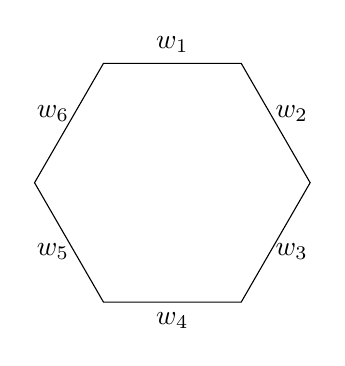
\begin{tikzpicture}
   \newdimen\R
\R=1.75cm
   \draw (0:\R)
   \foreach \x in {60,120,...,360} {  -- (\x:\R) }
 -- cycle (330:\R) node {$w_3$}
 -- cycle (270:\R) node {$w_4$}
 -- cycle (210:\R) node {$w_5$}
 -- cycle (150:\R) node {$w_6$}
 -- cycle  (90:\R) node {$w_1$}
 -- cycle  (30:\R) node {$w_2$};
\end{tikzpicture}
\caption{Sections of city walls}
\label{fig:city-walls}
\end{figure}

Given the scenario described above, as one could expect, the sentence in \ref{ex:explicit-partitives-wall-coll-italian} would be true if two parts of two distinct walls making up the complex were red, e.g., a part of $w_1$ and a part of $w_3$. But surprisingly, unlike \ref{ex:explicit-partitives-wall-pl-italian}, it would also be true if two distinct individual walls making up the complex were red, e.g., the wall $w_1$ and the wall $w_3$, or if two continuous sections of the walls making up the complex were red, e.g., the subsets $\{w_1, w_2\}$ and $\{w_4, w_5\}$. In other words, the meanings that are impossible in explicit set partitives with regular plurals, are easily available with irregular plurals. However, as already mentioned, there is a crucial constraint on possible interpretations of \ref{ex:explicit-partitives-wall-coll-italian}. Namely, one can count parts of the plurality consisting of the walls in question as one as long as they form a contiguous section of the whole structure, i.e., \ref{ex:explicit-partitives-wall-coll-italian} would not be true of two arbitrary pluralities constituted by walls that are not in a tangential relationship with each other. In particular, it would be false if, say, the wall $w_1$ as well as the walls $\{w_3, w_5\}$ were red.\footnote{I assume here the `exact $n$' interpretation of numerals (e.g., \citealt{horn1992said,geurts1998scalars,breheny2005some}; see also \citealt{geurts2006take} for an overview). Notice that the judgments do not change if the numeral is modified by overt \textit{exactly}.}\largerpage[2]

Likewise, assume a slightly morbid scenario involving a decaying human bone or skeleton and consider the contrasts between the examples in \ref{ex:explicit-partitives-bone-italian}.  

\ex.\label{ex:explicit-partitives-bone-italian} Italian (Enrico Flor, p.c.)
\ag. Tre   parti del    osso sono cariate.\label{ex:explicit-partitives-bone-sg-italian}\\
    three parts of.the bone are  decayed\\
    `Three parts of the bone are decayed.'
\bg. Tre parti degli ossi sono cariate.\label{ex:explicit-partitives-bone-pl-italian}\\
    three parts of.the bones are  decayed\\
    `Three parts of the bones are decayed.'
    \a. part-of-a-singularity reading
    \b. \#part-of-a-plurality reading
    \z.
\bg. Tre   parti delle  ossa sono cariate.\label{ex:explicit-partitives-bone-coll-italian}\\
    three parts of.the bones.\textsc{coll} are  decayed\\
    `Three parts of the skeleton are decayed.'
    \a. part-of-a-singularity reading
    \b. part-of-a-plurality reading
    \z.

Given that there is one relevant bone, the entity partitive in \ref{ex:explicit-partitives-bone-sg-italian} gets a part-of-a-singularity reading as usual, and thus the sentence would be true if there were three decayed spots on, e.g., a femur. This is not surprising and, similar to the interpretation of \ref{ex:explicit-partitives-bone-pl-italian}, fits the discussed semantic shift regarding modified explicit set partitives. However, the partitive involving the irregular plural \textit{ossa} in \ref{ex:explicit-partitives-bone-coll-italian} behaves differently. Seemingly, the most readily available interpretation of the example concerns three groups of connected bones making up the skeleton, e.g., it would be true of a decayed femur and knee, a decayed ulna and radius, and the decayed neck and skull. The sentence would be felicitous if three separate bones decayed though, e.g., a femur, ulna, and the skull. Furthermore, analogously to \ref{ex:explicit-partitives-bone-pl-italian} it would be judged true if there were decayed parts on three distinct bones, e.g., a part of the femur, a part of the ulna, and a part of the skull. But again, the reading that \ref{ex:explicit-partitives-bone-coll-italian} cannot get involves three collections of disconnected bones. For instance, it would be infelicitous in a scenario where, say, a femur and the skull, a radius and a knee, and a rib and an ankle bone are decayed. That is because these pairs of bones do not form cohesive wholes, i.e., topologically continuous entities of a particular sort, and consequently cannot be conceptualized as units one could quantify over.

\tabref{tab:properties-of-italian-parte} summarizes the patterns we have observed so far. Specifically, the quantificational behavior of the Italian part-word \textit{parte} depends on certain denotational properties of expressions it combines with. The labels `bare' and `count' in the table stand for bare explicit partitives and count explicit partitives, respectively, each of which can include a singular, a regular plural, or an irregular plural DP.

    \begin{table}[h]
    \centering
\begin{tabular}{lcccccc}
\lsptoprule
                           & \multicolumn{2}{c}{\textsc{singulars}}          & \multicolumn{2}{c}{\textsc{regular pl}}    & \multicolumn{2}{c}{\textsc{irregular pl}}  \\
                           & bare & count & bare & count & bare & count \\ \midrule
subatomic quantification   & $\checked$                   & $\checked$                    & *                              & $\checked$                    & $\checked$                   & $\checked$                    \\
quantification over wholes & *                              & *                               & $\checked$                   & *                               & $\checked$                   & $\checked$                    \\ \lspbottomrule
\end{tabular}
\caption{Properties of Italian \textit{parte} `part' in explicit partitives}
\label{tab:properties-of-italian-parte}
\end{table}

The investigation into the interaction between cardinal numerals and partitives involving Italian irregular plurals leads to a somewhat surprising conclusion. It turns out that the cross-linguistic observation concerning different properties of partitive words in entity and set partitives as discussed in \sectref{sec:partitivity-and-countability} actually does not provide evidence for distinct part-whole structures for singulars and plurals, as suggested by \citet{schwarzschild1996pluralities}. That is not to say that there is no difference in how constitution of objects as opposed to sums thereof is conceptualized. That is to say that the Italian data suggest that the difference does not regard the relation between parts and a whole, but rather that it regards the relation governing how parts are organized in space with respect to each other. In particular, regular plurals encode no topological relations between entities making up pluralities or, in other words, simply denote arbitrary sums of individuals. Consequently, parts of a plurality do not form an integrated entity that could be considered as a unit one could assign a number to, which seems to be a prerequisite for numerical quantification. On the other hand, despite the plurality inference, Italian irregular forms in \textit{-a} differ significantly from regular plurals and somewhat resemble singulars in that they do encode how parts are organized with respect to each other. Specifically, their extensions consist of cohesive aggregates, i.e., pluralities arranged in a particular spatial configurations such that individual objects making up a plurality are either connected or at least stay in a relatively stable proximity. Given that the domain of quantification consists of entities conceptualized as such clusters, counting parts consisting of several singularities is possible as long as they form integrated fragments or continuous sections of the whole. Therefore, I posit that the explanation of the patterns summarized in \tabref{tab:properties-of-partitive-words} and \ref{tab:properties-of-italian-parte} should be contingent on the manner how we conceptualize topological relations holding between parts of different types of entities as well as on the sensitivity of quantificational operations employed in natural language to such relations.

\section{Parts vs. subsets}\label{sec:parts-vs-subsets}

The Italian data provide intriguing evidence but let us hold on for a minute and reconsider the claim that being countable is a property of only those entities that are integrated wholes. One could wonder to what extent the fact that count explicit partitives involving regular plural DPs cannot quantify over sums and can only refer to parts of singular objects tells us anything about the nature of countability. After all, to the extent they are pragmatically admissible, sentences in which the cardinal modifies an expression such as \textit{subset} instead of a part-word are definitely compatible with an interpretation where the domain of quantification consists of collections of individuals, i.e., felicitous when counting subsets of a larger set. For instance, unlike \ref{ex:partitive-numeral-part-polish} the sentence in \ref{ex:partitive-numeral-subset-polish} would be true in a situation where there are, say, ten relevant apples $\{a_1, \dots, a_{10}\}$ and three arbitrary subsets of the apples got spoiled, e.g., $\{a_1, a_2\}$, $\{a_3, a_4, a_5\}$ and $\{a_6, a_7\}$.\footnote{This reading is different from a type of reading discussed in \sectref{sec:mass-parts-quantitifes-and-pieces} where reference to three-fourths of the total volume of the apples would be involved. What is crucial for the discussion of \ref{ex:partitive-numeral-part-polish} is that the quantified subsets of individuals cannot be arbitrary.} In other words, is it really the case that counting requires units that are integrated objects? Or maybe there is simply something weird about partitive words and we should not jump to a conclusion concerning countability based on the partitive data? 

\ex.\label{ex:partitive-numeral-subset-part-polish} Polish
\ag. Trzy podzbiory jabłek zgniły.\label{ex:partitive-numeral-subset-polish}\\
three subsets apples\textsc{.gen} rotted\\
`Three subsets of the apples got spoiled.'
\bg. Trzy części jabłek zgniły.\label{ex:partitive-numeral-part-polish}\\
three parts apples\textsc{.gen} rotted\\
`Three parts of the apples got spoiled.'
\a. part-of-a-singularity reading
\b. \#part-of-a-plurality reading
\z.

At first blush, this seems to be a justified objection and I think it should be taken seriously. However, there are a number of empirical facts suggesting that what happens in \ref{ex:partitive-numeral-subset-polish} is very different from what happens in \ref{ex:partitive-numeral-part-polish}. First of all, it is crucial to emphasize that natural language expressions such as \textit{set} or \textit{subset} are not merely linguistic reflections of set-theoretic concepts involving notions such as $\{\dots\}$ or relations $\subseteq$ and $\subset$. On the contrary, such expressions have a number of properties that classify them on a par with group nouns such as \textit{committee}, \textit{band}, or \textit{pile}.\footnote{In the following text, I will ignore the evidence for distinguishing between different classes of group nouns \citep[see][]{pearson2011new,henderson2017swarms,docekal_wagiel2018decomposing} and assume that for our purposes there are no relevant differences between nouns such as \textit{band} and \textit{pile}.} On the other hand, similarly to bare plurals set partitives refer to pluralities but part-words are not collectives, as attested by a number of tests involving predicate non-sharing. 

It has been proposed in the literature that group nouns and plural NPs do not co-refer since one can find multiple contrasts concerning (in)compatibility with certain predicates \citep{barker1992group,schwarzschild1996pluralities}. For instance, the sentence with a collective DP as a subject is perfectly fine with the predicate \textit{have five members}, see \ref{ex:collectives-members}, but its altered version involving a plural DP as in \ref{ex:plurals-members} is not.

\ex.\label{ex:collectives-plurals-members} English \citep[p. 153]{lonning1987mass}
\a. The committee has five members.\label{ex:collectives-members}
\b. \#The men have five members.\label{ex:plurals-members}

Now, let us test the behavior of the Polish part-word \textit{część} `part' with respect to plurals, regular collective nouns, and the expression \textit{podzbiór} `subset'.\footnote{It needs to be admitted that due to the restricted distribution of the noun \textit{podzbiór} (often limited to mathematical and computational contexts) the following sentences involving this expression is not how people usually talk. Rather, these examples sound nerdy or somewhat like clumsily worded math exercises rather than something a regular person would say. Nevertheless, despite the slight lexical oddity the judgments concerning compatibility with different predicates, interactions in co-variational contexts and with overt distributive operators seem to be rather clear.} The contrasts in \ref{ex:plurals-part-collectives-subset-polish-elements} show that bare plurals and bare explicit set partitives differ from the typical group noun \textit{stos} `pile' as well as \textit{podzbiór} in that they are not compatible with predicates of the type \textit{have ten elements}, which are assumed to indicate bunches \citep{schwarzschild1996pluralities}. 

\ex.\label{ex:plurals-part-collectives-subset-polish-elements} Polish
\ag. \#Jabłka składają się z dziesięciu sztuk.\label{ex:plurals-polish-elements}\\
apples consist \textsc{refl} from ten\textsc{.gen} items\textsc{.gen}\\
Intended: `The apples consist of ten items.'
\bg. \#Część jabłek składa się z dziesięciu sztuk.\label{ex:part-polish-elements}\\
part apples\textsc{.gen} consist \textsc{refl} from ten\textsc{.gen} items\textsc{.gen}\\
Intended: `Some of the apples consist of ten items.'
\bg. Stos jabłek składa się z dziesięciu sztuk.\label{ex:collectives-polish-elements}\\
pile apples\textsc{.gen} consist \textsc{refl} from ten\textsc{.gen} elements\textsc{.gen}\\
`The pile of apples consists of ten items.'
\bg. Podzbiór jabłek składa się z dziesięciu sztuk.\label{ex:subset-polish-elements}\\
subset apples\textsc{.gen} consist \textsc{refl} from ten\textsc{.gen} elements\textsc{.gen}\\
`The subset of apples consists of ten items.'

The same pattern can be observed when the examined expressions appear as first arguments of the two-place predicate \textit{należy do} `belongs to' which arguably designates assignment of objects to some abstract entity representing a collection. Though both \ref{ex:collectives-polish-belong} and \ref{ex:subset-polish-belong} are felicitous, the sentences including plurals and explicit set partitives in \ref{ex:plurals-polish-belong} and \ref{ex:part-polish-belong}, respectively, cannot saturate the predicate.

\ex.\label{ex:plurals-part-collectives-subset-polish-belong} Polish
\ag. \#Ta papierówka należy do jabłek.\label{ex:plurals-polish-belong}\\
this white.transparent belongs to apples\textsc{.gen}\\
Intended: `This white transparent apple belongs to the apples.'
\bg. \#Ta papierówka należy do części jabłek.\label{ex:part-polish-belong}\\
this white.transparent belongs to part\textsc{.gen} apples\textsc{.gen}\\
Intended: `This white transparent apple belongs to some of the apples.'
\bg. Ta papierówka należy do stosu jabłek.\label{ex:collectives-polish-belong}\\
this white.transparent belongs to pile\textsc{.gen} apples\textsc{.gen}\\
`This white transparent apple belongs to the pile of apples.'
\bg. Ta papierówka należy do podzbioru jabłek.\label{ex:subset-polish-belong}\\
this white.transparent belongs to subset\textsc{.gen} apples\textsc{.gen}\\
`This white transparent apple belongs to the subset of apples.'

Another contrast between plurals and collective nouns concerns distribution with reciprocals, as demonstrated in \ref{ex:reciprocals}. 

\ex.\label{ex:reciprocals} English \citep[p. 168]{schwarzschild1996pluralities}
\a. The rocks in that pile are touching each other.\label{ex:reciprocals-plural}
\b. \# That pile is touching each other.\label{ex:reciprocals-group}

Polish examples such as those in \ref{ex:plurals-part-collectives-subset-polish-reciprocals} show that there is a contrast between bare plurals and bare explicit set partitives, on the one hand, and typical collectives such as \textit{stos} and \textit{podzbiór}, on the other. 

\ex.\label{ex:plurals-part-collectives-subset-polish-reciprocals} Polish
\ag. Jabłka dotykają się nawzajem.\label{ex:plurals-polish-reciprocals}\\
apples touch \textsc{refl} each.other\\
`The apples are touching each other.'
\bg. Część jabłek dotyka się nawzajem.\label{ex:part-polish-reciprocals}\\
part apples\textsc{.gen} touches \textsc{refl} each.other\\
`Some of the apples are touching each other.'
\bg. \#Stos jabłek dotyka się nawzajem.\label{ex:collectives-polish-reciprocals}\\
pile apples\textsc{.gen} touches \textsc{refl} each.other\\
Intended: `The pile of apples touches each other.'
\bg. \#Podzbiór jabłek dotyka się nawzajem.\label{ex:subset-polish-reciprocals}\\
subset apples\textsc{.gen} touches \textsc{refl} each.other\\
Intended: `The subset of the apples touches each other.'

Plurals and explicit set partitives combine felicitously with reciprocal expressions, whereas collectives do not. In particular, \ref{ex:plurals-polish-reciprocals} and \ref{ex:part-polish-reciprocals} indicate either strong or intermediate reciprocity \citep{fiengo_lasnik1973logical,dalrymple1998reciprocal,beck2001reciprocals}, i.e., either each of the apples in question is touching all the other apples or any  two of the apples are connected by a chain of apples that  stand in the reciprocal relation. Nevertheless, it is impossible to define such truth conditions for \ref{ex:collectives-polish-reciprocals} and \ref{ex:subset-polish-reciprocals}.

A similar distribution is attested in contexts where the reciprocal is covert, see \ref{ex:covert-reciprocal}, including co-variational environments such as \ref{ex:covariation}. Specifically, plurals do combine with predicates triggering covariation, whereas group nouns do not. 

\ex.\label{ex:covert-reciprocal} English \citep{dougherty1970grammar}
\b.[] \# The trio collided. 

\ex.\label{ex:covariation} English \citep[p. 168]{schwarzschild1996pluralities}
\a. The members of group A live in different cities.\label{ex:covariation-plural}
\b. \# Group A lives in different cities.\label{ex:covariation-group}

Let us then consider Polish examples involving plurals, explicit partitives, group nouns, and phrases headed by \textit{podzbiór} in subject position, as provided in \ref{ex:covariation-polish} and \ref{ex:distributivity-polish}. In \ref{ex:covariation-polish-plural}, the sentence-internal \textit{different} expression \textit{w różnych miastach} `in different cities' is bound within a clause to express covariation with a plural argument due to a built-in distributive operator \citep{carlson1987same,beck2000semantics,brasoveanu2008sentence,dotlacil2010anaphora}. As a result, the sentence would be true if for each of the musicians it were the case that they lived in a city that is different from the cities other musicians live in. Due to this kind of meaning, sentence-internal \textit{different} expressions are good indicators of distributivity.\largerpage

    \ex. Polish\label{ex:covariation-polish} 
    \ag. Muzycy mieszkają w różnych miastach.\label{ex:covariation-polish-plural}\\
	musicians live in different\textsc{.loc} cities\textsc{.loc}\\
	`The musicians live in different cities.'
	\bg. Część muzyków mieszka w różnych miastach.\label{ex:covariation-polish-part}\\
	part musicians\textsc{.gen} lives in different\textsc{.loc} cities\textsc{.loc}\\
	`Some of the musicians live in different cities.'
	\bg. \# Zespół mieszka w różnych miastach.\label{ex:covariation-polish-group}\\
	band live in different\textsc{.loc} cities\textsc{.loc}\\
	Intended: `The band lives in different cities.'
    \bg. \# Podzbiór muzyków mieszka w różnych miastach.\label{ex:covariation-polish-subset}\\
	subset musicians\textsc{.gen} lives in different\textsc{.loc} cities\textsc{.loc}\\
	Intended: `A subset of the musicians lives in different cities.'

The sentences in \ref{ex:distributivity-polish} include the distributive preposition \textit{po} which is a marker for distant distributivity in Polish \citep[e.g.,][]{przepiorkowski2008generalised,przepiorkowski2010towards,przepiorkowski2014distance,przepiorkowski-patejuk2013syntax}.\footnote{For detailed studies on distant distributivity and distributive \textit{po} in Slavic see also, e.g., \citet{franks1994parametric,franks1995parameters}, \citet{harves2003getting}, and \citet{knezevic2015numerals}.} As such, similarly to binominal \textit{each} \citep[e.g.,][]{safir_stowell1988binominal,zimmermann2002boys,dotlacil2012binominal,champollion2012each} and distributive numerals \citep[e.g.,][]{gil2002distributive,oh2005plurality,cable2014distributive,hofherr_etxeberria2017distributive} \textit{po} marks the distributive share and distributes it over the distributive key denoted by a different phrase, here the subject DP. As a result, the possibility of a collective reading is ruled out and a sentence in which \textit{po} occurs is obligatorily interpreted distributively, e.g., in \ref{ex:distributivity-polish-plural} each of the musicians played a song. This conflicts with the semantics of group nouns which in general do not allow for the access to individual members of a collection, hence \ref{ex:distributivity-polish-group} is an awkward sentence. As witnessed by the contrast between \ref{ex:distributivity-polish-part} and \ref{ex:distributivity-polish-subset}, explicit set partitives pattern with plurals, whereas \textit{podzbiór} behaves as typical collectives.

	\ex. Polish\label{ex:distributivity-polish}
    \ag. Muzycy zagrali po piosence.\label{ex:distributivity-polish-plural}\\
	musicians played \textsc{distr} song\textsc{.loc}\\
	`The musicians played a song each.'
	\bg. Część muzyków zagrała po piosence.\label{ex:distributivity-polish-part}\\
	part musicians\textsc{.gen} played \textsc{distr} song\textsc{.loc}\\
	`Some of the musicians played a song each.'
	\bg. \# Zespół zagrał po piosence.\label{ex:distributivity-polish-group}\\
	band played \textsc{distr} song\textsc{.loc}\\
	Intended: `The band played a song each.'
    \bg. \# Podzbiór muzyków zagrał po piosence.\label{ex:distributivity-polish-subset}\\
	subset musicians\textsc{.gen} played \textsc{distr} song\textsc{.loc}\\
	Intended: `A subset of the musicians played a song each.'
    
Yet another diagnostic involves the VP disjunction test proposed by \citet[pp. 30--31]{de_vries2015shifting}. When the test is applied, \textit{część} does not exhibit the kind of behavior associated with group nouns. To illustrate this, let us consider the sentences in \ref{ex:vp-disjunction-plural}.

\ex. English \citep[p. 31; adapted]{de_vries2015shifting}
\a. The children are singing or dancing.\label{ex:vp-disjunction-plural}
\a. collective reading\label{ex:vp-disjunction-plural-coll}
\b. distributive reading\label{ex:vp-disjunction-plural-distr}
\z.
\b. The team is singing or dancing.\label{ex:vp-disjunction-group}
\a. collective reading\label{ex:vp-disjunction-group-coll}
\b. \#distributive reading\label{ex:vp-disjunction-group-distr}
\z.

In \ref{ex:vp-disjunction-plural}, the definite plural DP \textit{the children} serves as a subject of the disjunctive sentence. There are two possible interpretations of \ref{ex:vp-disjunction-plural}. On the collective interpretation, see \ref{ex:vp-disjunction-plural-coll}, the disjunction \textit{singing or dancing} holds of the plurality as a whole. In other words, it is either the case that all the relevant children are singing or that all the relevant children are dancing. However, there is yet another reading of \ref{ex:vp-disjunction-plural}, namely the distributive interpretation, see \ref{ex:vp-disjunction-plural-distr}, according to which the disjoined VPs hold not of the plurality of children as a whole but rather of each individual child. Thus, some of the children might be singing while others might be dancing. Crucially, when the definite plural is replaced with a group noun such as \textit{team} as in \ref{ex:vp-disjunction-group}, the distributive interpretation is no longer available. The only reading such a sentence can get is that the whole plurality was either involved in singing or in dancing.

Now, let us examine the behavior of Polish nouns \textit{część} and \textit{podzbiór} compared to plurals and group nominals in sentences involving VP disjunction such as those in \ref{ex:vp-disjunction-polish}. 
	
	\ex.\label{ex:vp-disjunction-polish} Polish
    \ag. Dzieci tańczą lub śpiewają.\label{ex:vp-disjunction-polish-plural}\\
	children dance or sing\\
	`The children are dancing or singing.'
	\a. collective reading
	\b. distributive reading
	\z.
	\bg. Grupa dzieci tańczy lub śpiewa.\label{ex:vp-disjunction-polish-group}\\
	group children\textsc{.gen} dances or sings\\
	`The group of children is dancing or singing.'
	\a. collective reading
	\b. \#distributive reading
	\z.
	\bg. Część dzieci tańczy lub śpiewa.\label{ex:vp-disjunction-polish-part}\\
	part children\textsc{.gen} dances or sings\\
	`Some children are dancing or singing.'
	\a. collective reading
	\b. distributive reading
    \z.
   \pagebreak\bg. Pozbiór dzieci tańczy lub śpiewa.\label{ex:vp-disjunction-polish-subset}\\
   subset children\textsc{.gen} dances or sings\\
   `A subset of children is dancing or dancing.'
   	\a. collective reading
	\b. \#distributive reading
    \z.

The example \ref{ex:vp-disjunction-polish-plural} can have either a collective or a distributive reading, i.e., it would be true either when all the children are dancing or singing or when some are dancing whereas others are singing. On the other hand, a sentence with a group noun as a subject like \ref{ex:vp-disjunction-polish-group} can only be interpreted collectively. That is also the case in \ref{ex:vp-disjunction-polish-subset}, i.e., all the children in the relevant subset need to be either dancing or singing. However, \ref{ex:vp-disjunction-polish-part} is felicitous in both collective and distributive scenarios. Once again, the \textit{part} word \textit{część} patterns with plurals rather than collectives, which definitely proves that it differs from expressions such as \textit{subset}.

Notice that whatever theory of the relationship between agreement and collectivity/distributivity one might have (e.g., \citealt{de_vries2015shifting}; see also \citealt{schwarzschild1996pluralities} and \citealt{pearson2011new} for the discussion of group nouns in British English as well as  \citealt{bosnic2016distributivity} for experimental data concerning distributivity and agreement mismatches in BCS), it cannot explain the semantic difference between \textit{part} expressions and group nouns. In Polish, \textit{część} just like \textit{zespół} (and any other group noun) triggers singular agreement on the verb. As witnessed by the glosses in the examples provided above, in sentences with both explicit partitives and group nouns, see \ref{ex:covariation-polish-part}--\ref{ex:covariation-polish-group} and \ref{ex:vp-disjunction-polish-group}--\ref{ex:vp-disjunction-polish-part}, the verbs agree in number with the subjects. Furthermore, both in \ref{ex:distributivity-polish-part} and \ref{ex:distributivity-polish-group} the past participles agree with \textit{część} and \textit{zespół} in gender by taking the feminine and masculine form, respectively. Therefore, it is not the agreement pattern but rather lexical properties of \textit{część} that are accountable for the semantic difference.

Finally, despite being distinct syntactic categories partitive words pattern with cardinal numerals in that in general they allow for modification by class A/B modifiers such as \textit{more than} and \textit{at least} \citep{nouwen2010two,nouwen2016plurality,brasoveanu2012modified}, see \ref{ex:partitives-polish-modifiers}.\footnote{Since there are some restrictions in this respect which I believe result from the indefinite nature of some partitive words, I present here only parallel examples with class B modifiers.} This again suggests that their semantics includes a purely quantificational component.

\ex.\label{ex:partitives-polish-modifiers} Polish
\ag. {Co najmniej} część murów jest czerwona.\label{ex:explicit-partitives-polish-at-least} \\
at.least part walls\textsc{.gen} is red\\
`At least some of the walls are red.'
\bg. {Co najwyżej} część murów jest czerwona.\label{ex:explicit-partitives-polish-at-most} \\
at.most part walls\textsc{.gen} is red\\
`At most some of the walls are red.'
\bg. {Co najmniej} połowa murów jest czerwona.\label{ex:proportional-partitives-polish-at-least} \\
at.least half walls\textsc{.gen} is red\\
`At least half of the walls are red.'
\bg. {Co najwyżej} połowa murów jest czerwona.\label{ex:proportional-partitives-polish-at-most} \\
at.most half walls\textsc{.gen} is red\\
`At most half of the walls are red.'
\bg. {Co najmniej} pięć murów jest czerwonych.\label{ex:count-partitives-polish-at-least} \\
at.least five walls\textsc{.gen} is red\\
`At least five of the walls are red.'
\bg. {Co najwyżej} pięć murów jest czerwonych.\label{ex:count-partitives-polish-at-most} \\
at.most five walls\textsc{.gen} is red\\
`At most five of the walls are red.'

The results of a battery of tests applied to the Polish nouns \textit{część} `part' and \textit{podzbiór} `subset' unequivocally indicate that \textit{podzbiór} is a group noun,\footnote{\citeauthor{schwarzschild1996pluralities} (\citeyear[p. 168]{schwarzschild1996pluralities}) actually lists \textit{set} among group nouns.} and thus triggers obligatory collective interpretations of sentences in which it occurs, whereas \textit{część} patterns with plurals including being ambiguous between collective and distributive readings. This is a significant contrast between the expressions in question suggesting that their extensions differ in a significant way. In particular, it has been commonly advocated in the literature that group nouns do not refer to pluralities but rather to atomic individuals, i.e., somewhat abstract singularities that might be associated with their members \citep[e.g.,][]{barker1992group,schwarzschild1996pluralities,winter2001flexibility,champollion2017parts}.\footnote{But see, e.g., \citet{link1984hydras,link1998algebraic}, \citet{landman1989groupsi,landman1989groupsii,landman2000events}, and \citet{de_vries2015shifting} for an alternative view on which a group noun denotes a special type of plurality shifted to an impure atom or group-atom depending on a particular approach. \citet{pearson2011new}, on the other hand, proposes that group nouns are predicates of individual concepts.} Whatever extraordinary properties such atoms have, it is plausible to assume that they are conceptualized as something distinct from mere sums of objects.

Therefore, I conclude that explicit partitives refer to genuine pluralities where\-as group nouns including expressions such as \textit{set} and \textit{subset} denote abstract entities that are associated with pluralities of their members but are ontologically distinct from them. Having this in mind, there is nothing surprising about the fact that count explicit set partitives do not quantify over sums of individuals, and in fact, it turns out that part-words actually pattern with regular nominals, as will be shown below. 

It has been observed for a long time that the semantics of numeral phrases in languages such as English poses a compositional puzzle. On the one hand, cardinal numerals higher than \textit{one} combine only with plural nominals, on the other, plural NPs modified by cardinals are interpreted as singular expressions. Specifically, although plurals denote sums of entities, the domain of quantification is always a set of atomic individuals (\citealt{kratzer1989investigation}; \citealt{chierchia1998reference}; \citealt{landman2000events}; see also \citealt{kobuchi-philip2006identity}). Contrary to what one would expect if numerals simply counted elements in a given set \citep[e.g.,][]{barwise_cooper1981generalized} and combined with plural nouns in a straightforward manner, cardinals seem to be sensitive only to singular individuals in the sense that they do not assign numbers to sums of objects. Actually, this fact has already been realized in the system of \citet{link1983logical} where the extension of a phrase such as \textit{three children} is supposed to contain only special types of elements, namely exactly three atoms. To illustrate why such a restriction is necessary, let us consider the sentence in \ref{ex:domain-of-quantification-example}.   

\ex.\label{ex:domain-of-quantification} \a. Three children slept.\label{ex:domain-of-quantification-example}		
	 \b. $\llbracket \text{children} \rrbracket = \{a, b, c, d, ab, ac, ad, bc, bd, cd, abc, abd, acd, bcd, abcd\}$\label{ex:domain-of-quantification-numeral-phrase}
     \b. $\llbracket \text{three children} \rrbracket \cap \llbracket \text{slept} \rrbracket = \{a, ab, abcd\}$\label{ex:domain-of-quantification-wrong-meaning1}
     \b. $\llbracket \text{three children} \rrbracket \cap \llbracket \text{slept} \rrbracket = \{a, b, ab\}$\label{ex:domain-of-quantification-wrong-meaning2}

Let us assume that there are four relevant children in the universe of discourse, say, Anne, Betty, Carl, and Danny, i.e., $a$, $b$, $c$, and $d$ respectively. Then the meaning of the plural noun \textit{children} is the set involving both atomic children and all the sums generated by joining the atoms, see \ref{ex:domain-of-quantification-numeral-phrase}. If \textit{three} simply counted the elements in the set denoted by the modified noun, among the possible verifications of the sentence in \ref{ex:domain-of-quantification-example} would be \ref{ex:domain-of-quantification-wrong-meaning1} and \ref{ex:domain-of-quantification-wrong-meaning2} since in both cases the set of children that slept consists of three elements.

The truth conditions in \ref{ex:domain-of-quantification-wrong-meaning1} and \ref{ex:domain-of-quantification-wrong-meaning2} predict \ref{ex:domain-of-quantification-example} to be true both in a scenario where there were four individual children sleeping and in a scenario where only two individual children slept. However, this not how the sentence is understood. It seems that what cardinals in a language such as English do is that they restrict possible verifications of sentences including numeral phrases in such a way that sums of individuals are excluded from the domain of quantification.\footnote{Alternatively, one might assume that there is a null classifier responsible for this restriction \citep[e.g.,][]{selkirk1977some,kobuchi-philip2006identity}.} 

With this in mind, let us return to count explicit partitives such as the Italian examples in \ref{ex:count-explicit-partitives-italian}, repeated here as \ref{ex:count-explicit-partitives-italian2}. Similarly to regular plural DPs, unmodified explicit set partitives denote pluralities or, more precisely, sub-pluralities. However, when combined with a numeral they do not allow for quantification over sub-pluralities but only over material parts of individuals making up pluralities.  

\ex.\label{ex:count-explicit-partitives-italian2} Italian \citep[p. 186; adapted]{schwarzschild1996pluralities}
\ag. tre parti del muro\label{ex:count-explicit-entity-partitives-italian2}\\
three parts of.the wall\\
`three parts of the wall'
\bg. tre parti dei muri\label{ex:count-explicit-set-partitives-italian2}\\
three parts of.the walls\\
`three parts of the walls'
\a. part-of-a-singularity reading
\b. \#part-of-a-plurality reading
\z.

At first blush, it seems surprising but actually in languages such as English the same effect can be found in numeral phrases. Specifically, the numeral combines with the plural noun which denotes a set of pluralities; however, the domain of quantification does not consist of pluralities but rather atomic individuals. Hence, as demonstrated in \ref{ex:count-explicit-partitives-numeral-phrases} the phrase \textit{three walls} does not mean three pluralities of walls but rather a plurality of three walls. Likewise, the Italian partitive phrase in \ref{ex:count-explicit-set-partitives-italian2} cannot be interpreted as three pluralities of sub-pluralities of walls. Instead, it would be felicitously paraphrased as a plurality of three parts of walls.

		\ex. Pluralities of wholes and parts\label{ex:count-explicit-partitives-numeral-phrases}
        \a. three walls
		\a. \#three pluralities of walls
		\b. plurality of three walls
        \z.
        \b. tre parti dei muri
		\a. \#three pluralities of parts-of-a-plurality of walls
		\b. plurality of three parts of walls
		\z.
		
In this section, I argued that set partitives differ from collectives and discussed a number of issues regarding the domain of quantification in count explicit partitives as well as group nouns and plurals modified by cardinal numerals. An important question that arises after examining the evidence explored in this chapter is why natural language does not allow for counting a sum of entities as one thing unless it satisfies certain topological (or other) criteria. 

\section{Summary}\label{sec:summary-ch2}

The data discussed in this chapter provide compelling evidence that cross-linguis\-tically it is common for the same partitive word including proportional quantifiers such as half-words to appear both in entity and set partitives. This fact suggests that such expressions can operate both at the superatomic and subatomic level depending on what structure is provided by the embedded DP. Furthermore, on the basis of the zeugma test involving German partitives with conjoined singular and plural DPs I showed that it is empirically inadequate to account for the parallelism between explicit and proportional entity and set partitives in terms of semantic ambiguity. 

However, at the same time explicit partitives modified by a cardinal numeral can only quantify over material parts of singular individuals irrespective of \linebreak whether the complement DP is singular or plural. At first sight, this fact seems to be at variance with the claim that there is unified parthood utilized by partitive words in both entity and set partitives. Nonetheless, an important empirical finding concerning Italian irregular plurals showed that if a plural expression encodes a certain topological configuration, i.e., denotes entities conceptualized as cohesive pluralities, count explicit partitives can get a part-of-a-plurality reading in such a case. This fact demonstrates that the uncountability of explicit partitives with plurals does not indicate per se different part-whole structures for singularities and pluralities. Rather, countability results from the interplay between the meaning of a partitive word and the extension of a singular or plural DP it combines with, and topological constraints play a crucial role in this interaction.

Given the cross-linguistic and intra-linguistic evidence explored in this chapter, the two remaining possibilities are the following. It is either the case that singulars and plurals employ a unified part-whole structure or that their mereologies do differ but at the same time partitive words involve a derived indeterminate notion of parthood which allows them to quantify over elements of whatever part-whole structure they are applied to. I argue for the first option. However, by advocating this claim I do not advance a view that singulars and plurals employ the same structures. What I claim is that it is not the part-whole relation that differs but rather that there is another notion involved which is responsible for how parts are topologically arranged with respect to each other. Intuitively, this seems correct since we conceptually distinguish between integrated wholes and arbitrary sums of parts, and quantification in natural language is sensitive to the distinction. Specifically, only things conceptualized as integrated parts of integrated wholes can be assigned numbers when counting. On the other hand, scattered entities such as pluralities are prohibited from the domain of quantification cardinal numerals establish unless certain individuation criteria are satisfied. In addition, Italian irregular plurals provide evidence that there are natural language expressions involving yet another type of structure. In particular, such nominals designate entities that are similar to plurals in that they consist of multiple integrated objects, but at the same time the sum thereof is arranged in a particular way, i.e., it constitutes a cluster.

So far, I have argued that explicit and proportional partitives provide evidence that countability is restricted to entities that form an integrated whole as typically denoted by concrete singular count nouns, while the arbitrary sums of parts regular plural nouns refer to cannot be counted. Furthermore, the data concerning subatomic quantification suggests that this constraint is also applicable at the level of material parts of individuals. If that is correct, one would expect that there are natural language expressions dedicated exclusively to quantification over integrated parts similar to cardinal numerals that count integrated wholes. In the next section, I will introduce novel data concerning distinct types of half-words in Polish as well as other partitive expressions.
